\documentclass{article}
\usepackage{graphicx}%
\usepackage{multirow}%
\usepackage{amsmath,amssymb,amsfonts}%
\usepackage{amsthm}%
\usepackage{mathrsfs}%
\usepackage[title]{appendix}%
\usepackage{xcolor}%
\usepackage{textcomp}%
\usepackage{manyfoot}%
\usepackage{booktabs}%
\usepackage{algorithm}%
\usepackage{algorithmicx}%
\usepackage{algpseudocode}%
\usepackage{listings}%




\usepackage{tikz}%draw graphs
\usepackage{pgfplots}
\pgfplotsset{compat=1.18}

\usepackage{float}%make tables stay?



\providecommand{\keywords}[1]{\textbf{\textit{Keywords: ---}} #1}%keywords

\usepackage{parskip} %puts \noindent everywhere

\usepackage[font=small,labelfont=bf]{caption}
\usepackage{subcaption}

%\usepackage{caption}
%\DeclareCaptionFormat{citation}{%
%  \ifx\captioncitation\relax\relax\else
%    \captioncitation\par
%  \fi
%  #1#2#3\par}
%\newcommand*\setcaptioncitation[1]{\def\captioncitation{\textit{Source:}~#1}}%to add sources to figures
%\let\captioncitation\relax
%\captionsetup{format=citation,justification=centering}

%https://www.overleaf.com/project/642180d8a08db24a02633ac7


\usepackage{hyperref} 
% Hyperref setup
\hypersetup {
    colorlinks=true,
    urlcolor=blue,
    linkcolor=black,
    filecolor=black,  
    citecolor=black,
}

\usepackage{apacite}

\raggedbottom
%%\unnumbered% uncomment this for unnumbered level heads

%\usepackage[margin=1.25in]{geometry}

\usepackage{geometry}
\geometry{
 a4paper,
 total={150mm,257mm},
 left=30mm,
 top=20mm
}

\usepackage[swedish,english]{babel}


\begin{document}

\title{\huge \vfill \scshape{Optimal TSP Solvers: Time-Constrained Algorithm Analysis}}
\author{
    \small \scshape{Harry Zhang} \\ 
    \small \scshape{Supervisors: Per-Olof Freerks and Felicia Dinnetz} \\
    \scriptsize \scshape{Kungsholmens Gymnasium}
    \\
    
\includegraphics[scale=0.3]{docs/pictures/KGlogopng.png}
    \\
}
\maketitle
\vfill


\thispagestyle{empty} 
\newpage

\begin{center}
    \textbf{Abstrakt}
\end{center}
\noindent Denna studie undersöker handelsresandeproblemet (TSP) på det Euklidiska planet, vilket är känt som ett NP-fullständigt problem. Olika heuristiska algoritmer och strategier används vanligtvis för att tackla detta problem. I denna artikel jämförs fyra olika heuristiska algoritmer: slumpmässig generering, modifierad Dijkstras algoritm, slumpmässig omplacering och 2-opt-omplacering. Målet är att identifiera den algoritm som kan producera den mest optimala lösningen inom en tidsbegränsning på 2 sekunder. För att bedöma deras prestanda testas alla algoritmer på olika testfall. Varje algoritm körs sex gånger på 10 olika testfall med varierande storlek, fördelning och egenskaper. Resultaten avslöjar flera relevanta fynd. Framför allt presterar 2-opt-algoritmen konsekvent bättre än de andra tre algoritmerna och ger övergripande sett de mest optimala lösningarna. Det är dock värt att notera att den modifierade Dijkstras algoritmen utmärker sig i scenarier där den optimala vägen nära följer naturliga rutter. Samtidigt presterar slumpmässig omplacering konsekvent sämre än 2-opt-algoritmen, medan slumpmässig generering visar sämst prestanda av de fyra algoritmerna. All kod finns tillgänglig vid \href{https://github.com/hairez/diploma-project}{https://github.com/hairez/diploma-project}.

\textbf{\textit{Nyckelord}:} handelsresandeproblemet, euklidiska avstånd, grafer, heuristiska algoritmer


\thispagestyle{empty}
\newpage

\begin{center}
    \textbf{Abstract}
\end{center}
\noindent This study investigates the Traveling Salesman Problem (TSP) on the Euclidean plane, which is known to be an NP-complete problem. Various heuristic algorithms and strategies are commonly employed to tackle this problem. In this paper, four distinct heuristic algorithms are compared: random generation, modified Dijkstra's algorithm, random swapping, and 2-opt swapping. The aim is to identify the algorithm that can produce the most optimal solution within a 2-second time constraint. To assess their performance, all algorithms are tested on different test cases. Each algorithm is executed six times on 10 diverse test cases, featuring varying sizes, distributions, and traits. The obtained results reveal several key findings. Primarily, the 2-opt algorithm consistently outperforms the other three algorithms, yielding the most optimal solutions overall. However, it is noteworthy that the modified Dijkstra's algorithm excels in scenarios where the optimal path closely aligns with natural pathways. Conversely, the random swapping algorithm consistently performs worse than the 2-opt algorithm, while the random generation algorithm exhibits the poorest performance among the four algorithms. The codes are available at \href{https://github.com/hairez/diploma-project}{https://github.com/hairez/diploma-project}.

\textbf{\textit{Keywords}:} travelling salesman problem, Euclidean distance, graph, heuristic algorithms



\thispagestyle{empty} 
\newpage

\tableofcontents
\thispagestyle{empty}
\setcounter{page}{0}
\newpage

\section{Introduction}\label{Introduction}

\subsection{Background}\label{Background}
Consider a salesman that wants to visit a number of cities around the world. The salesman does not have to visit the cities in any particular order, but after the salesman has visited all the desired cities, the salesman has to return to the city it started out in. The salesman is also only allowed to visit each city once, with the exception of the city that it started out in, which the salesman is allowed to leave once and enter once. It is fairly straightforward how to find any path that works, but what is the path with the shortest Euclidean distance$_{\ref{Euclidean distance}}$ that visits all the cities and returns to the initial starting position?
This is the problem statement of the classic problem called \textit{The travelling salesman problem}, but it is also called \textit{the travelling salesperson problem}, or just \textit{TSP} for short.

\begin{figure}[ht]
 \centering
 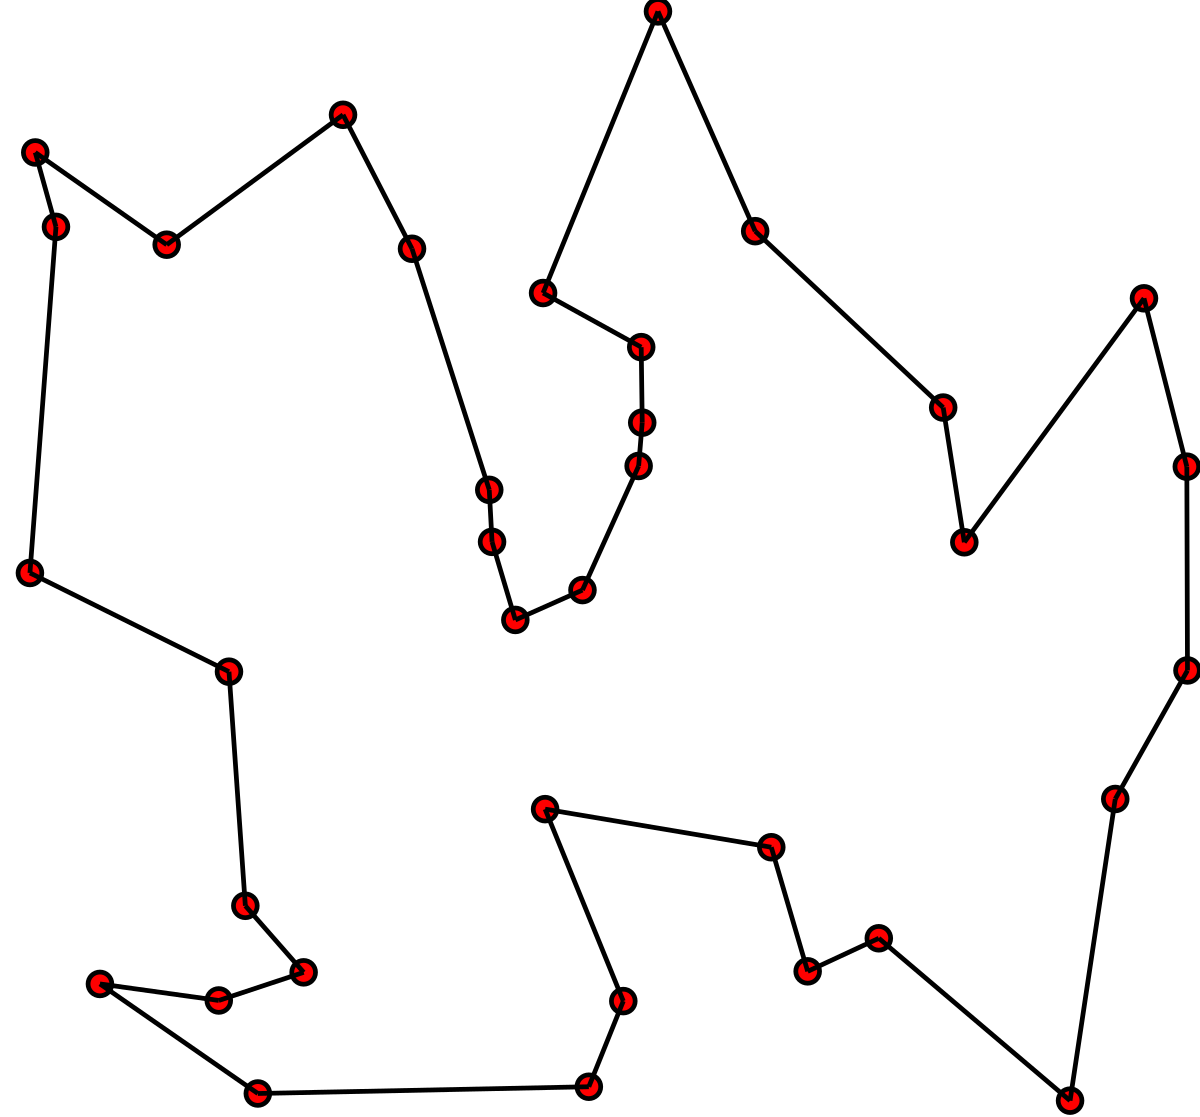
\includegraphics[scale=.15]{docs/pictures/tsp.png}
 \caption{TSP interpreted as a graph where a path is found. \cite{wiki:TSP}}
 \label{Figure:TSP-as-graph}
\end{figure}

\noindent
The travelling salesman problem could also be interpreted as a weighted undirected graph$_{\ref{undirected weighted graph}}$ with some number of nodes. Each node represents a city that the travelling salesman has to visit. The edges between each pair of nodes have a specific value or length, which signifies the Euclidean distance between that pair of cities. Given any $2$ cities, the distance from city A to city B is always the same as the distance from city B to city A.
\newline
Variations of the traveling salesman problem exist \cite{gutin_punnen_2007}, however, the version where the goal is to minimize the distance in Euclidean space is currently an NP-complete$_{\ref{NP-complete}}$ problem \cite{PAPADIMITRIOU1977}. 
\newline
Evidence shows that there exist no algorithms that could find the definite shortest path in polynomial time, at the same time as there are no algorithms that can guarantee any accuracy in any given Map with cities. However, there are algorithms that can guarantee solutions that will be some constant number factor within the optimal solution \cite{Christofides}. Other than that, verifying if any specific path is the most optimal is also unmanageable. \cite{PAPADIMITRIOU1977}
\newline
For example, a brute force solution could be considered to solve the classic travelling salesman problem, where all possible permutations of the order are computed, and then picking the shortest path out of all possible paths. Although this would be applicable to a smaller number of cities, the number of permutations possible would have a factorial$_{\ref{factorial}}$ growth the more cities that are required to be visited. 
\newline
It is an NP-hard problem and there are a lot of different heuristic$_{\ref{Heuristic}}$ algorithms. Some algorithms are more efficient in some situations than others. In this research, different algorithms are going to be tested on different test cases within a set amount of time. The algorithms being tested in this paper are a random generation algorithm, a modified Dijkstra's algorithm, a genetic algorithm with random swapping, and a genetic algorithm with 2-opt swapping.
\newline
The relevance and application of the travelling salesman problem in the real world such as optimizing routes for delivery vehicles, robots, or public transportations to minimize the travel distances, reduce fuel costs, and improve overall efficiency. The travelling salesman problem could also be applied to more technical concepts, such as finding the most optimal way to drill a circuit board or finding the most efficient order for sequencing genetic material such as DNA. 

\subsection{Aim}\label{Aim}
The aim of this paper is to find the limits of different heuristic algorithms for solving the travelling salesman problem. 

\subsection{Research Question}\label{RQ}
What algorithm out of the random generation algorithm, a modified Dijkstra's algorithm, the random swapping algorithm, and the 2-opt swapping are most efficient in finding the shortest path in a weighted graph, in a set amount of time?



\subsection{Theory}\label{Theory}

\subsubsection{Notations and definitions}\label{Notation and definitions}

This section explains a list of basic mathematical and computer scientific definitions and terms. 
\newline

\begin{enumerate}   %use the following to refer back to this part:
                    %$_{\ref{Polynomial}}$
 
  \item The \textbf{\textit{Euclidean distance}} between two points $p_1=(x_1,y_1)$ and $p_2=(x_2,y_2)$ is defined as $\sqrt{(x_2-x_1)^2+(y_2-y_1)^2}$. \label{Euclidean distance}
  \item An \textbf{\textit{undirected weighted graph}} is a type of graph where edges connect vertices, and each edge has an associated weight or cost. In an undirected graph, the edges do not have a specified direction, meaning they can be traversed in both directions.\label{undirected weighted graph}
  \item A problem is \textbf{\textit{NP-complete}} if no efficient algorithm is currently known that, could solve all instances of the problem in a reasonable amount of time. The term "complete" in NP-complete signifies that these problems are among the hardest problems in the class NP. If an efficient algorithm can be found for any NP-complete problem, it would imply that efficient algorithms exist for all problems in NP, which is considered highly unlikely. \label{NP-complete}
  \item The \textbf{\textit{factorial}} of a given non-negative integer $n$ is denoted by "$n!$". It is the product of all positive integers less than or equal to $n$.$$n! = n \cdot (n-1) \cdot (n-2) \cdot ... \cdot 2 \cdot 1 .$$\label{factorial}
  \item A \textbf{\textit{logarithm}} is a mathematical function that represents the exponent to which a given base must be raised to produce a specific number. In other words, it provides a way to reverse the process of exponentiation. $$b^x=a \Leftrightarrow \log_b{a}=x.$$ In computer science, logarithms with base 2 are commonly used because they align with binary representation and the binary logarithm.  In this paper, whenever logarithms are mentioned, they will always be considered to be with base 2.\label{logarithm}
  
  \item The \textbf{\textit{triangle inequality}} states that for any three points $A$, $B$, and $C$ in a space, the distance between $A$ and $C$ is always less than or equal to the sum of the distances between $A$ and $B$, and between $B$ and $C$. Another way to interpret the triangle inequality is by drawing a triangle, and observing how each side of the triangle will always be shorter or equal in length to the sum of the other $2$ sides. \label{Triangle Inequality}
  
    \begin{figure}[ht]
     \centering
     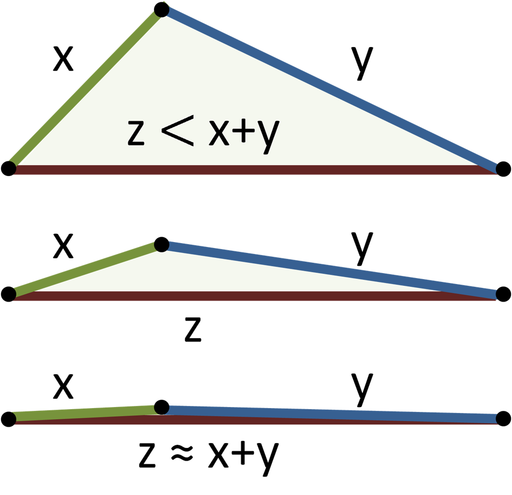
\includegraphics[scale=0.3]{docs/pictures/TriangleInequality.png}
     \caption{Examples of the triangle inequality for triangles with the side-lengths $x$, $y$, and $z$. \cite{wiki:Triangle}}
     \label{Figure:TriangleInequality}
    \end{figure}
    
\end{enumerate}




\subsubsection{Big O Notation}\label{Big O}
When computer scientists want to compare different kinds of algorithms, they can describe the efficiency of the algorithm with a mathematical function that describes the estimated run time of the algorithm using Big O notation. Big O notation is a way of describing the time complexity of an algorithm, which refers to how long an algorithm takes to complete based on the size of its input. The big O notation shows a huge difference when comparing the worst-case scenarios for each algorithm.
\newline
The ``O'' in Big O notation stands for ``order of magnitude'', which means that the function described grows a the same rate or within a constant factor as the function that is given. Hence when describing time complexities using big O notation, the coefficient becomes irrelevant. For example, an algorithm such as calculating the roots of a quadratic equation takes a constant time regardless of the size of the coefficients and has a time complexity of $O(1)$, even though the algorithm could possibly perform more than $1$ operation. If the time complexity of an algorithm grows linearly with the size of the input, the time complexity of the algorithm would be $O(n)$. An example of an algorithm with a linear time complexity would be to calculate the sum of an array with $n$ integers. The algorithm would be required to iterate through the whole array, as long as no other sum using this array has been pre-computed. Some other examples of common time complexities are: $O(\log{n})$, $O(n \log{n})$, $O(n^2)$, $O(2^n)$, and $O(n!)$.

\subsubsection{Heuristic Algorithms}\label{Heuristic}
When trying to solve a computational problem, it is crucial to find a relatively fast approach that is both efficient in finding the most optimal solution and in a short period of time, especially when a large amount of input is considered. A common rule of thumb within competitive programming is to always use a program that performs less than $10^7$ operations.
\newline
As mentioned in the background, a brute force solution trying all possible paths for the travelling salesman problem would take an exceeding number of operations to compute. The time complexity of a brute force solution would be $O(n!)$, which means that it would be a sufficient enough algorithm if the number of cities would be less or equal to $10$, since $10! = 3628800 < 10^7$ and $11! > 10^7$. Any Map with more than $10$ cities would take a lot more time before stopping to compute, while Maps with more than $1000$ would not even stop computing after several years.
\newline
When the optimal solution is either unknown or computationally infeasible to find within a reasonable time frame, heuristic algorithms are used instead to provide an approximate solution. These algorithms prioritize efficiency and practicality over exact optimality. In this research, several different heuristic algorithms are used to repeatedly find the shortest path for the travelling salesman problem, and all the heuristic algorithms used will have a time complexity that is either $O(n)$ or $O(n \log{n})$. This also implies that Maps with up to $10^6$ cities could be experimented on these algorithms without spending an unreasonable amount of time waiting for the algorithms to stop computing.
\newline
The heuristic algorithms compared to solve the travelling salesman problem in this research are:
\begin{itemize}
  \item Random generation algorithm.
  \item A modified version of Dijkstra's Algorithm.
  \item Genetic Algorithm with Random Swapping.
  \item Genetic Algorithm with 2-opt swapping.
\end{itemize}


\subsubsection{Random Generation Algorithm}\label{Random}
The random generation algorithm generates a random permutation of all possible nodes and calculates the length of the path generated. It always stores the path with the shortest path and repeats this algorithm until the time limit is reached. The algorithm is similar to repeatedly throwing some amount of dice, and after each throw the sum of all the results is stored. The more dice there are, the smaller the probability for the throw to result in the highest number possible.

\begin{algorithm}[H]
\caption{Random path generator}
\begin{algorithmic}

\While{Less than 2 seconds has passed}
    \State $order \gets $ random permutation of the $n$ nodes
    \State $currPath \gets calculatePath(order)$ \Comment{\textcolor{blue}{$calculatePath(array)$ returns the length of the whole path}}
    \If{$bestPath > currPath$}
        \State $bestOrder \gets order$
        \State $bestPath \gets currPath$
    \EndIf
\EndWhile
\State $\textbf{print } bestOrder $
\State $\textbf{print } bestPath $

\end{algorithmic}
\end{algorithm}

\noindent
This algorithm has a time complexity of $O(n)$, since the generation of a random path has to iterate through each possible city. One assumption could be made for the random generation algorithm, which is that it is very unlikely for it to find the most optimal path when there are a lot of cities. Especially when no other optimization is applied to make the path shorter. However, for Maps with less number of cities, it is likely for the algorithm to randomly find the best path within a reasonable time limit. Similarly, for any number of cities, as long as enough time is given for the algorithm, it would eventually find the shortest path. Nevertheless, in that case, where the algorithms could run for an infinite amount of time, the brute force solution would always guarantee to find the shortest solution.

\subsubsection{Modified Dijkstra's Algorithm}\label{Dijkstras}
Dijkstra's algorithm is an algorithm used on weighted, directed graphs with non-negative weights. Dijkstra's algorithm will find the shortest path between a source node and all other nodes in a weighted graph. The algorithm maintains a priority queue of nodes and repeatedly selects the node with the smallest known distance from the source. It then updates the distances of its neighboring nodes, considering the weights of the edges. This process continues until all nodes have been visited, and the shortest path from the source to each node is determined. It can find a relatively short path within a reasonable time limit, but it is not guaranteed to find the shortest path. In some way, Dijkstra's algorithm could be visualized as always picking the shortest path between two given nodes in the graph. Furthermore, the original Dijkstra's algorithm is used on a directed graph, starting from a source node and ending on any other node in the graph. However, that is not the case of the travelling salesman problem.

\noindent
A modified version of Dijkstra's algorithm could be applied to the travelling salesman problem instead. Given a starting node, iterate through all other unvisited nodes and find the shortest distance. This process is repeated on the node that had the shortest distance from the previous node until all nodes have been visited. 

\noindent
It might seem that this approach will always find the shortest path, however, there are cases where this approach does not do that. 

\begin{figure}[ht]
     \centering
     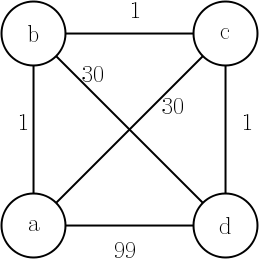
\includegraphics[scale=0.5]{docs/pictures/dijkstras.png}
     \caption{Example of a graph where the modified Dijkstra's algorithm would not find the shortest path.}
     \label{Figure:CounterExampleDijkstras}
\end{figure}
\noindent
For example in Figure \ref{Figure:CounterExampleDijkstras}, always choosing the closest neighbor would not provide the optimal path for this graph. If the salesman started on the node $a$, by repeatedly choosing the closest unvisited node it would city, it would traverse the graph by going $a \rightarrow b \rightarrow c \rightarrow d \rightarrow a$ which would result in a path with a cost of 102. There is a path with a lower cost, which is to go $a \rightarrow b \rightarrow d \rightarrow c \rightarrow a$, which would have a cost of 62 instead. One reason explaining why this algorithm cannot always find the most optimal path is that algorithms are required to find a path that returns from the starting position. Since the modified Dijkstra's algorithm is fundamentally only looking one step forward for each iteration, choosing whatever is the best option at the moment without considering the future consequences.

\noindent
Furthermore, this version of Dijkstra's algorithm's time complexity would be $O(n^2)$, since for each node, the distance to all other nodes has to be calculated. However, by only comparing the $\log{n}_{\ref{logarithm}}$ random neighbors, and going to the closest one out of those, this modified Dijkstra's algorithm would essentially become an algorithm with a time complexity of $O(n \log{n})$. 

\begin{algorithm}[H]
\caption{Modified Dijkstra's algorithm for $\log{n}$ neighbors}
\begin{algorithmic}

\While{Less than 2 seconds has passed}
    \State $currOrder \gets $ empty list 
    \State $unvisted \gets $ random permutation of the $n$ nodes \Comment{\textcolor{blue}{$unvisited$ is a list}}
    \State $currOrder.append(unvisited.pop())$

    \For {$i = 0 \text{ to } n-1 $} 
        \State $bestNeighbor \gets unvisited[-1]$ 
        \State $closest \gets \infty $
        \State $focus \gets $ empty list  


        \State $focusSize \gets min(length(unvisited),ceil(\log{n}))$ \Comment{\textcolor{blue}{All remaining neighbors will be checked if there are less than $\log{n}$ neighbors left}}

        \For {$j = 0 \text{ to } focusSize $}
            \State $focus.append(unvisited.pop())$ \Comment{\textcolor{blue}{$focus$ will contain the $\log{n}$ random neighbors}}
        \EndFor

        \For {$j = 0 \text{ to } focusSize $}
            \State $currDist \gets distance(currOrder[-1],focus[j])$ 
            \If{currDist < closest}
                \State $closest \gets currDist$
                \State $bestNeighbor \gets focus[j]$
            \EndIf
        \EndFor

        \State $currOrder.append(bestNeighbor)$

        \For {$j = 0 \text{ to } focusSize $}
            \If{$focus[j] != bestNeighbor$}
                \State $unvisited.append(focus[j])$ \Comment{\textcolor{blue}{Put back all the unvisited cities to $unvisited$}}
            \EndIf
        \EndFor
    \EndFor
    \State $currPath \gets calculatePath(currOrder)$
    \If{$bestPath > currPath$}
        \State $bestOrder \gets currOrder$
        \State $bestPath \gets currPath$
    \EndIf
\EndWhile

\State $\textbf{print } bestOrder $
\State $\textbf{print } bestPath $

\end{algorithmic}
\end{algorithm}


\noindent
Undeniably, by only checking with $\log{n}$ random neighbors would not give an as optimal answer as checking with all neighbors. However, on a Map with a lot of cities where many cities share the same a similar distance to another city, the probability is very high for the algorithm to pick one of those neighbors as one of the $\log{n}$ random neighbors, which would give a result very similar to the algorithm that checks with all neighbors.





\subsubsection{Genetic Algorithm with Random Swapping}\label{Random Swapping}
Genetic algorithms can be used as general-purpose optimization algorithms. They are inspired by the process of natural selection and genetics, and they are widely used for solving optimization problems in various domains. Some common uses of genetic algorithms are in machine learning, neural networks, and engineering to find the most optimal parameters for different designs. \cite{YANG202191} Other than that, they can also be used in combinatorial optimization problems such as the travelling salesman problem. 

\noindent
The way a genetic algorithm commonly function is similar to the principles of evolution. The algorithm starts by creating a population with several potential solutions to the problem, where each solution could be represented as a set of parameters or even a chromosome. By applying a fitness function to each individual solution in the population, each solution can be evaluated on how well it can solve the problem. In the next generation of solutions, the solutions with the best fitness from the previous generation are chosen to be the parents of the new solutions. Mutations of the parents will be created, at the same time as the worse performing solutions will be removed from the population. This will be repeated, which results in a population consisting of several high-performing solutions. 

\noindent
The version of the genetic algorithm used in this research will essentially use the same principle as the one described. This genetic algorithm with random swapping starts off with a randomly generated path. After that, two cities in this path will be repeatedly randomly chosen. Using the current neighbors of those cities it is possible to calculate the change in the distance, if the nodes were to be swapped. If this creates a longer path than before, then the nodes are not swapped. However, if the change would make the path shorter, then the nodes are swapped. This repeats until no improvements have been made after 4000 randomly chosen pairs of cities.

\noindent
It is even possible to evaluate if the change would benefit the path can be done in a constant number of operations because it is only necessary to compare the neighboring cities of the two randomly chosen cities.
\begin{figure}[ht]
     \centering
     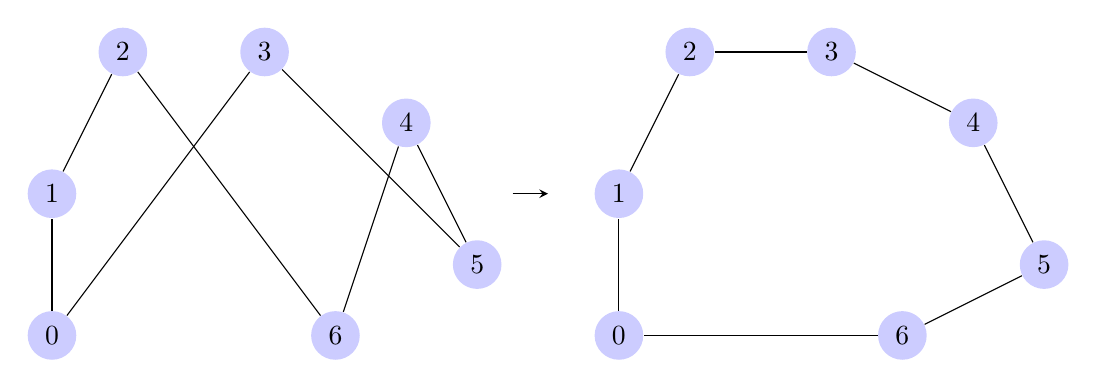
\begin{tikzpicture}  
  [scale=.9,auto=center,every node/.style={circle,fill=blue!20}] % here, node/.style is the style pre-defined, that will be the default layout of all the nodes. You can also create different forms for different nodes.  
    \centering 

    \node (a0) at (0,3)     {0};  
    \node (a1) at (0,5)     {1};
    \node (a2) at (1,7)     {2};  
    \node (a6) at (3,7)     {3};  
    \node (a4) at (5,6)     {4};  
    \node (a5) at (6,4)     {5};  
    \node (a3) at (4,3)     {6};

    \draw (a0) -- (a1);
    \draw (a1) -- (a2);  
    \draw (a2) -- (a3);  
    \draw (a3) -- (a4);  
    \draw (a4) -- (a5);  
    \draw (a5) -- (a6);  
    \draw (a6) -- (a0);

    \draw [-stealth](6.5,5) -- (7,5);

    \node (b0) at (8,3)     {0};  
    \node (b1) at (8,5)     {1};
    \node (b2) at (9,7)     {2};  
    \node (b3) at (11,7)     {3};  
    \node (b4) at (13,6)     {4};  
    \node (b5) at (14,4)     {5};  
    \node (b6) at (12,3)     {6};

    \draw (b0) -- (b1);
    \draw (b1) -- (b2);  
    \draw (b2) -- (b3);  
    \draw (b3) -- (b4);  
    \draw (b4) -- (b5);  
    \draw (b5) -- (b6);  
    \draw (b6) -- (b0);  
  
\end{tikzpicture} 
     \caption{Example of a path that has been improved by swapping the order of two cities.}
     \label{Figure:Swapping}
\end{figure}

\noindent
In Figure \ref{Figure:Swapping}, the order of city $3$ and city $6$ has been swapped. Notice how the edges $0 \rightarrow 1$, $1 \rightarrow 2$, $4 \rightarrow 5$ remain unchanged. The reason for that is that only city $3$ and city $6$ would get affected by the swap, which means that only the edges connected to the cities being swapped have to be considered. This also implies that, if the sum of the lengths of the edges affected has decreased, it would mean that the swap leads to a shorter path.

 

\begin{algorithm}[H]
\caption{Random Swapping}
\begin{algorithmic}

\While{Less than 2 seconds has passed}
    \State $currOrder \gets $ random permutation of the $n$ nodes

    \State $steps \gets 0$ \Comment{\textcolor{blue}{keeps track of the number of times cities have been compared without any improvements}}

    \While{Less than 2 seconds has passed}
        \State $steps \gets steps + 1$
        \State $x \gets $ random number from 0 to n-1 \Comment{\textcolor{blue}{index of a random city in $currOrder$}}
        \State $y \gets $ random number from 0 to n-1

        \State $distBefore \gets segmentDist(x) + segmentDist(y)$ \Comment{\textcolor{blue}{$segmentDist(x)$  returns the distance from the city in $currOrder$ before $x$ to $x$ + distance from $x$ to the city in $currOrder$ after $x$}}

        \State $distAfter \gets swappedDist(x,y) + segmentDist(y,x)$ \Comment{\textcolor{blue}{$swappedDist(x,y)$  returns the distance from the city in $currOrder$ before $x$ to $y$ + distance from $y$ to the city in $currOrder$ after $x$}}

        \If{$distAfter < distBefore$}
            \State $steps \gets 0$
            \State $currOrder[x],currOrder[y] \gets currOrder[y],currOrder[x]$ \Comment{\textcolor{blue}{swap index $x$ and $y$}}
        \ElsIf{$steps > 4000$}
            \State \textbf{break}
        \EndIf
    \EndWhile

    \State $currPath \gets calculatePath(currOrder)$
    \If{$bestPath > currPath$}
        \State $bestOrder \gets currOrder$
        \State $bestPath \gets currPath$
    \EndIf
\EndWhile

\State $\textbf{print } bestOrder $
\State $\textbf{print } bestPath $

\end{algorithmic}
\end{algorithm}

\noindent
The algorithm required $O(n)$ to generate a random permutation of the cities. After that, it only performs a constant number of operations for each swap, which means $O(1)$ for each evaluation or swap. This repeats until 2 seconds have gone by.

\noindent
There are many advantages to a genetic algorithm since it will continuously try to improve a given solution. However, at some point, it will stop improving, since it will have reached a local optimum, which means that there are no other improvements that could be made by only swapping two cities. Eventually, it would require a bigger modification in the path for the path to become even shorter, which also implies that this algorithm cannot guarantee the optimal solution for any Map either. \cite{YANG202191}

\subsubsection{Genetic Algorithm with 2-opt swapping}\label{2-opt swapping}
The genetic algorithm with 2-opt swapping is another genetic algorithm, but instead of swapping two random nodes, it will swap two random edges. It is similar to the genetic algorithm with random swapping$_{\ref{Random Swapping}}$, since this algorithm also starts off with a randomly generated path. Afterward, two edges are repeatedly randomly chosen. Using the nodes the edges are connected to, the change in distance can be simulated and evaluated. If this creates a longer path compared to before, then the edges are not swapped. However, if the change would make the path shorter, then the edges are swapped. This also repeats until no improvements have been made after 4000 randomly chosen pairs of edges.


\begin{figure}[ht]
     \centering
     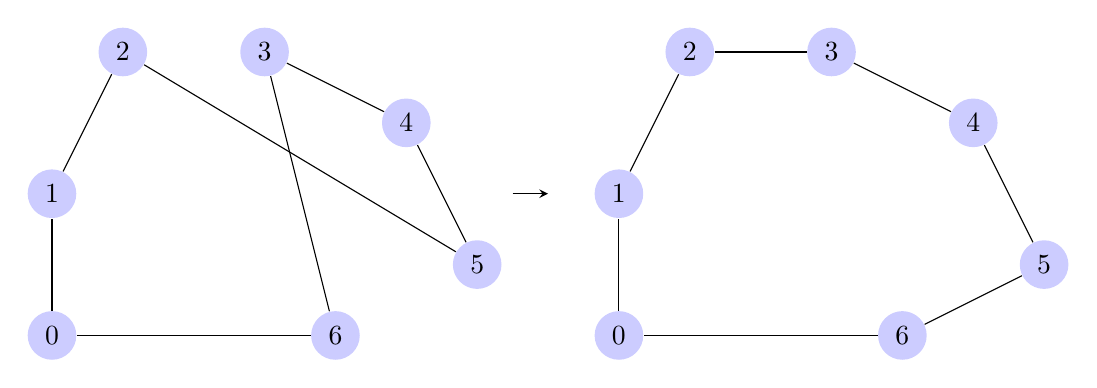
\begin{tikzpicture}  
  [scale=.9,auto=center,every node/.style={circle,fill=blue!20}] % here, node/.style is the style pre-defined, that will be the default layout of all the nodes. You can also create different forms for different nodes.  
    \centering 

    \node (a0) at (0,3)     {0};  
    \node (a1) at (0,5)     {1};
    \node (a2) at (1,7)     {2};  
    \node (a3) at (3,7)     {3};  
    \node (a4) at (5,6)     {4};  
    \node (a5) at (6,4)     {5};  
    \node (a6) at (4,3)     {6};

    \draw (a0) -- (a1);
    \draw (a1) -- (a2);  
    \draw (a2) -- (a5);  
    \draw (a3) -- (a4);  
    \draw (a4) -- (a5);  
    \draw (a3) -- (a6);  
    \draw (a6) -- (a0); 

    \draw [-stealth](6.5,5) -- (7,5);

    \node (b0) at (8,3)     {0};  
    \node (b1) at (8,5)     {1};
    \node (b2) at (9,7)     {2};  
    \node (b3) at (11,7)     {3};  
    \node (b4) at (13,6)     {4};  
    \node (b5) at (14,4)     {5};  
    \node (b6) at (12,3)     {6};

    \draw (b0) -- (b1);
    \draw (b1) -- (b2);  
    \draw (b2) -- (b3);  
    \draw (b3) -- (b4);  
    \draw (b4) -- (b5);  
    \draw (b5) -- (b6);  
    \draw (b6) -- (b0);  
  
\end{tikzpicture} 
     \caption{Example of a path that has been improved by replacing two of the edges.}
     \label{Figure:2opt}
\end{figure}

\noindent
This algorithm is called 2-opt because two edges are randomly chosen, as opposed to another algorithm called 3-opt, where three edges are randomly chosen. The ``opt'' in 2-opt and 3-opt stands for optimization. 

\noindent
Notice that there is only one possible way for the edges to be replaced so the new graph is not similar to the previous one, and for the graph to stay connected.


\noindent
It can also be proven that whenever two edges cross each other, it will always be shorter to swap the edges. This can be proven using the triangle inequality$_{\ref{Triangle Inequality}}$, since when two edges cross each other, two triangles that are missing one side each are created. By replacing the edges, the existing sides of the triangle will be replaced by the non-existing sides, which will guarantee a shorter path, if not equal length. This is shown in Figure \ref{Figure:triangleIneq2opt}.

\begin{figure}[ht]
     \centering
     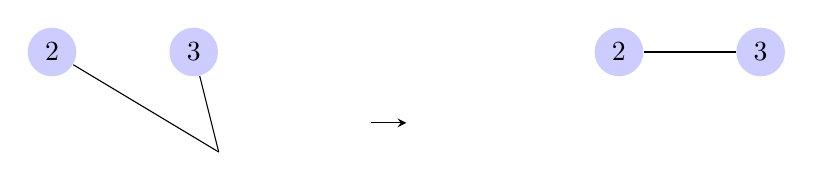
\begin{tikzpicture}  
  [scale=.9,auto=center,every node/.style={circle,fill=blue!20}] % here, node/.style is the style pre-defined, that will be the default layout of all the nodes. You can also create different forms for different nodes.  
    \centering 


    \node (a2) at (1,7)     {2};  
    \node (a3) at (3,7)     {3};   

    \draw (a2) -- (57/17,5.588235);  
    \draw (a3) -- (57/17,5.588235);  


    \draw [-stealth](5.5,6) -- (5.5+0.5,6);

    \node (b2) at (9,7)     {2};  
    \node (b3) at (11,7)     {3};   

    \draw (b2) -- (b3);  
  
\end{tikzpicture} 
     \caption{Example of how the triangle inequality could be visualized when edges are replaced in a path.}
     \label{Figure:triangleIneq2opt}
\end{figure}

\noindent
In other words, if there are edges that cross each other, they would eventually be replaced by more optimal edges that make the total path shorter.

\begin{algorithm}[H]
\caption{Random 2-opt swapping}
\begin{algorithmic}

\While{Less than 2 seconds has passed}
    \State $currOrder \gets $ random permutation of the $n$ nodes

    \State $steps \gets 0$ 

    \While{Less than 2 seconds has passed}
        \State $steps \gets steps + 1$
        \State $x \gets $ random number from $0$ to $n-2$ 

        \State $y \gets $ random number from $x+1$ to $n-$1 \Comment{\textcolor{blue}{to make sure the two unique edges are picked}}


        \State $xLeft \gets $ city in $currOrder$ before $x$
        \State $yRight \gets $ city in $currOrder$ after $y$

        
        \State $distBefore \gets distance(currOrder[x], xLeft) + distance(currOrder[y], yRight)$ 

        \State $distAfter \gets distance(currOrder[x], yRight) + distance(currOrder[y], xLeft)$ 

        \If{$distAfter < distBefore$}
            \State $steps \gets 0$
            \State reverse the sub-array of $currOrder$ from index $x$ to $y$.
        \ElsIf{$steps > 4000$}
            \State \textbf{break}
        \EndIf
    \EndWhile

    \State $currPath \gets calculatePath(currOrder)$
    \If{$bestPath > currPath$}
        \State $bestOrder \gets currOrder$
        \State $bestPath \gets currPath$
    \EndIf
\EndWhile

\State $\textbf{print } bestOrder $
\State $\textbf{print } bestPath $

\end{algorithmic}
\end{algorithm}

\noindent
The process of replacing the edges would in the worst-case scenario require a traverse of the whole array, which means one replacement would in the worst-case scenario be linear $O(n)$ in time complexity. At the same time in the best-case scenario, it would be for the algorithm to not replace, which would only take a constant number $O(1)$ of operations. For that reason, the genetic algorithm with random 2-opt swapping would have a higher constant factor compared to random swapping with nodes. The same reasoning could be used when comparing the efficiency of 2-opt with 3-opt. Because if three edges are considered, there are many more ways to replace the edges.

\noindent
The algorithm requires $O(n)$ to generate an initial random permutation of the cities. After that, the algorithm performs up to $O(n)$ operations for each replacement of edges. This repeats until 2 seconds have gone by.

\noindent
The way the 2-opt algorithm untangles crossing edges would efficiently decrease the total path of a random path, especially since the requirements for the edges to be replaced is only that the sum of the length of the new edges is shorter than the edges before. However, identically to random node swapping, this algorithm would also reach a local optimum. This also implies that this algorithm cannot guarantee to find the optimal solution.


\subsubsection{Maps}\label{Maps}
In this research, 10 Maps were generated. Some Maps were randomly generated to fit some kind of shape, while others were based on actual Maps from real countries such as Sweden and the United States of America.

\noindent
The Maps generated are numbered from 1 to 10, and the following is a small description of each Map.

\begin{enumerate}
  \item 10 uniformly randomized cities.
  \item 1000 uniformly randomized cities.
  \item 10000 uniformly randomized cities.
  \item 1916 different cities in Sweden.
  \item 49 locations in the United States of America. All states but Hawaii and Alaska are included. District of Columbia is included.
  \item 10000 randomized cities where all points are strictly increasing. 
  \item 10000 randomized cities, but the points form a circle.
  \item 10000 cities placed all integer coordinates from 1 to 100.
  \item 10000 randomized cities, but all the points share the same $y$-coordinate.
  \item 100 randomized cities where all points are strictly increasing.
\end{enumerate}

\noindent
Maps 1, 2, and 3 consist of cities with coordinates that are uniformly chosen. Map 4 is based on real coordinates of cities existing in Sweden. The data for Map 4 is taken from a GitHub repository \cite{SwedishCities}. Map 5 is based on 48 American states and the District of Columbia. Hawaii and Alaska are not included because those states are considered to be located relatively far away from all other states. The data for Map 5 is taken from Dataset Publishing Language powered by Google \cite{DatasetUSA}. Maps 6 and 10 consist of randomly chosen coordinates, but the coordinates of the points are strictly increasing. This means that for any two points $p_1 = (x_1,y_1)$ and $p_2=(x_2,y_2)$ on Maps 6 and 10, if $x_1 < x_2$ fulfilled, then $y_1 < y_2$ is also true. In Map 7 all the points form a circle. Map 8 creates a "grid" where most cities have 4 cities that are neighboring and closest. Map 9 essentially creates a straight line. All of the test data used are visualized in the appendix \ref{appendix:TestData}. The exact test data can also be found at \href{https://github.com/hairez/diploma-project/tree/main/code/tsp/data/secret}{https://github.com/hairez/diploma-project/tree/main/code/tsp/data/secret}.



\subsubsection{Integers and Floats}\label{Int VS Float}
Integers and floats are two primary data types for representing numbers in computer programming. Integers are used specifically for storing whole numbers, while floats are designed to handle decimal numerals. However, when it comes to processing float numbers, computers are generally known for their relative inefficiency compared to working with integers. For this reason, all coordinates of the Maps are rounded to the nearest integer, even though coordinates on a real Map are not necessarily integers. On the other hand, calculating the Euclidean distance$_{\ref{Euclidean distance}}$ requires the use of a square root, which could result in the distance being non-integer. If the distance would be rounded, it could potentially lead to an inaccurate result. For that reason, the distances of the paths are kept as floats. 




\section{Methodology}\label{Methodology}
\subsection{Method}\label{Method}
Firstly, $10$ different Maps with various numbers of cities were generated$_{\ref{Maps}}$. The $10$ different Maps with test data were run on $4$ separate algorithms that were made to solve the traveling salesman problem using Euclidean distance. The algorithms used were: Random generation algorithm$_{\ref{Random}}$, Modified Dijkstra's algorithm$_{\ref{Dijkstras}}$, Genetic algorithm with random swapping$_{\ref{Random Swapping}}$, and Genetic algorithm with 2-opt swapping$_{\ref{2-opt swapping}}$. All algorithms were written in Python 3, and all tests were run on Python version 3.10.6 64-bit. Both the algorithms and the results could be found on \href{https://github.com/hairez/diploma-project/tree/main/code/tsp}{https://github.com/hairez/diploma-project/tree/main/code/tsp}. Each Map was tested with each algorithm $6$ times, resulting in $6$ replicates of each combination of Map and algorithm. Several replicates were made since a factor of randomness is involved in each algorithm. For each execution of the algorithm, a time limit was set to a maximum of 2 seconds. After all runs, the paths found were recorded as well as the length of the path. The results were later compared across different Maps.

\noindent
The constant variables of this method are the various Maps, the time limit, computer hardware, and the programming language used, which was Python 3. The independent variable is the algorithm used for each replicate, and the dependent variable is the length of the shortest path found using these algorithms.


\subsection{Limitations}\label{Limitations}
One limitation is the scope of algorithms used. This study only considers $4$ algorithms for solving the travelling salesman problem. However, there could be other algorithms that are not included in the study which could perform better in a similar time-constrained environment. Similarly, combinations of these algorithms are also possible to create and could in the same way also be a more optimal option than the algorithms used. 

\noindent
At the same time, the algorithms used in the study may require more fine-tuning on various parameters to achieve even more optimal performance. 

\noindent
The results of the study may be dependent on the hardware and software used for the experiments. The same algorithms may perform differently using different hardware or with different compilers.

\noindent
Another limitation is the different Maps used. Since only $10$ different Maps are being considered here, it would not represent fully all possible scenarios. 

\noindent
These limitations should be taken into consideration before drawing any generalized conclusion from the results of these Maps.


\section{Results}\label{Results}
\subsection{Raw Results}
After 6 runs of each combination of algorithm and Map, the results were recorded. The raw results can be found in appendix \ref{appendix:RawResults}. The value in the results represents the length in length units. The lower the value is, the shorter the path.


\subsection{Processed Results}

The mean and standard deviation are given in Tables \ref{Table 1} and \ref{Table 2}.


\begin{table}[H]
    \caption{Mean and standard deviations of the raw results for each algorithm for Maps 1 to 5. Random generation algorithm, modified Dijkstra's algorithm, genetic random swapping algorithm, and genetic 2-opt swapping algorithm are mentioned. The values are distance values, and all values are given in units of length.}\label{Table 1}
    \centering
    \begin{tabular}{|l|l|l|l|l|l|}
    \hline
        ~ & Map 1 & Map 2 & Map 3 & Map 4 & Map 5 \\ \hline
        Random Gen Mean & 5931611.347 & 990989576.9 & 10297662286 & 79693630.34 & 63502.61492 \\ \hline
        Random Gen StDev & 98071.37382 & 2802386.561 & 15005360.31 & 0 & 2016.200921 \\ \hline
        Modified Dijkstra's Mean & 5891573.876 & 372698762.9 & 3234113811 & 27621763.38 & 31675.87155 \\ \hline
        Modified Dijkstra's StDev & 0 & 2240105.103 & 3959723.497 & 108885.9355 & 588.4132446 \\ \hline
        Random Swapping Mean & 5891573.876 & 225115031.8 & 3811725120 & 19706392.59 & 22647.95397 \\ \hline
        Random Swapping StDev & 0 & 9689780.489 & 23965143.87 & 377031.2052 & 1255.940382 \\ \hline
        2-opt Swapping Mean & 5891573.876 & 70079398.91 & 3040000568 & 6025155.901 & 18275.29668 \\ \hline
        2-opt Swapping StDev & 0 & 1291505.509 & 77298161.28 & 132900.3136 & 44.92499363 \\ \hline
    \end{tabular}
\end{table}


\begin{table}[H]
    \caption{Mean and standard deviations of the raw results for each algorithm for Maps 6 to 10. Random generation algorithm, modified Dijkstra's algorithm, genetic random swapping algorithm, and genetic 2-opt swapping algorithm are mentioned. The values are distance values, and all values are given in units of length.}\label{Table 2}
    \centering
    \begin{tabular}{|l|l|l|l|l|l|}
    \hline
        ~ & Map 6 & Map 7 & Map 8 & Map 9 & Map 10 \\ \hline
        Random Gen Mean & 9302983636 & 12570216770 & 515270.6256 & 6544965739 & 68743594.1 \\ \hline
        Random Gen StDev & 15207604.31 & 18812568.95 & 888.9918074 & 21588586.7 & 1108871.265 \\ \hline
        Modified Dijkstra's Mean & 1351063859 & 2238808383 & 162280.1463 & 951472838.7 & 20858190.36 \\ \hline
        Modified Dijkstra's StDev & 3547948.175 & 11170657.25 & 418.5181522 & 6157343.039 & 491755.728 \\ \hline
        Random Swapping Mean & 2332111751 & 3912911804 & 186698.2714 & 1630940997 & 11513068.17 \\ \hline
        Random Swapping StDev & 35083492.44 & 39740072.84 & 1610.624947 & 31710622.62 & 749593.063 \\ \hline
        2-opt Swapping Mean & 1618529033 & 2532409238 & 147065.8208 & 830152879.7 & 5805784.202 \\ \hline
        2-opt Swapping StDev & 115784019.8 & 78817208.42 & 2344.771193 & 55194184.9 & 8549.426892 \\ \hline
    \end{tabular}
\end{table}


\begin{figure}[H]
    \centering
    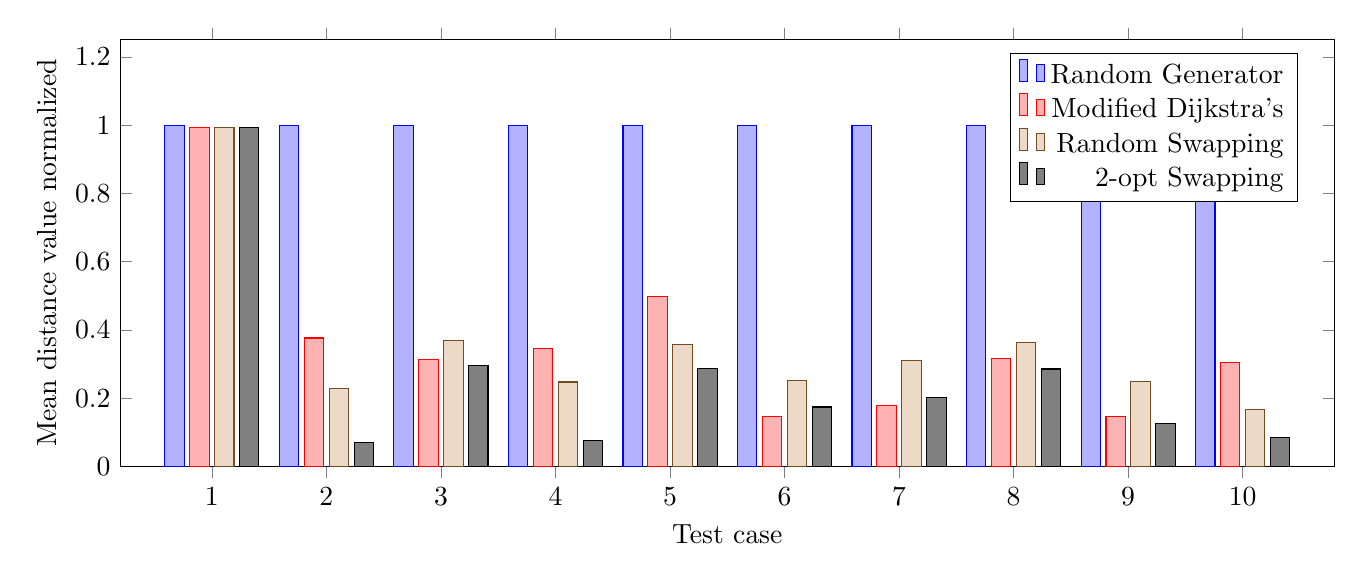
\begin{tikzpicture}
        \begin{axis} [
            ybar,
            bar width = 7pt,
            width = 17cm,
            height = 7cm,
            xlabel = Test case,
            ylabel = Mean distance value normalized,
            xmin = 1,
            xmax = 10,
            ymin = 0,
            ymax = 1,
            legend cell align={right},
            legend pos = north east,
            %x tick label style={rotate=45},
            xtick = data,
            %ytick = data,
            y tick label style={/pgf/number format/1000 sep=},
            enlarge y limits = {value = .25, upper},
            enlarge x limits = {abs = .8}
            %enlarge x limits = {abs = .8}
        ]
        \addplot+ [
                error bars/.cd,
                    y dir=both,
                    % (changed from `y explicit` so the error bars are (clearly) visible
                    y explicit ,
            ] coordinates {
                (1, 1) 
                (2, 1) 
                (3, 1) 
                (4, 1)
                (5, 1) 
                (6, 1) 
                (7, 1) 
                (8, 1) 
                (9, 1) 
                (10, 1) 
            };
        \addplot+ [
                error bars/.cd,
                    y dir=both,
                    % (changed from `y explicit` so the error bars are (clearly) visible
                    y explicit ,
            ] coordinates {
                (1, 0.9932501527) 
                (2, 0.3760874702) 
                (3, 0.3140629127) 
                (4, 0.3465993864)
                (5, 0.4988120819) 
                (6, 0.1452290912) 
                (7, 0.1781041986) 
                (8, 0.3149415826) 
                (9, 0.1453747623) 
                (10, 0.3034201314) 
            };

        \addplot+ [
                error bars/.cd,
                    y dir=both,
                    % (changed from `y explicit` so the error bars are (clearly) visible
                    y explicit ,
            ] coordinates {
                (1, 0.9932501527) 
                (2, 0.2271618562) 
                (3, 0.3701544112) 
                (4, 0.2472768841)
                (5, 0.3566460059) 
                (6, 0.2506842796) 
                (7, 0.3112843538) 
                (8, 0.3623305155) 
                (9, 0.2491901504) 
                (10, 0.1674784149) 
            };

        \addplot+ [
                error bars/.cd,
                    y dir=both,
                    % (changed from `y explicit` so the error bars are (clearly) visible
                    y explicit ,
            ] coordinates {
                (1, 0.9932501527) 
                (2, 0.07071658526) 
                (3, 0.2952126884) 
                (4, 0.07560398334)
                (5, 0.2877880967) 
                (6, 0.1739795636) 
                (7, 0.2014610634) 
                (8, 0.285414719) 
                (9, 0.1268383843) 
                (10, 0.08445563951) 
            };
        \legend {Random Generator, Modified Dijkstra's, Random Swapping, 2-opt Swapping};
        \end{axis}
    \end{tikzpicture}
\caption{Bar graph displaying the means of each algorithm on each Map from 1-10. All means are normalized to the mean of the results of the random generator algorithm.} \label{MeanDiagram}
\end{figure}

\noindent
In Figure \ref{MeanDiagram}, the smaller the bar is, the better the algorithm performed. Figure \ref{MeanDiagram} together with Tables \ref{Table 1} and \ref{Table 2} shows that the 2-opt swapping algorithm is the best-performing algorithm out of the used algorithms in the majority of the test cases. Modified Dijkstra's is also shown to be performing the best out of all algorithms used on Maps 6 and 7. 

%\subsection{Statistical Tests}

\section{Discussion}\label{sec4}

\subsection{Generalized Results}\label{subsec1}
When the number of cities is sufficiently small, all algorithms will find the shortest path possible given 2 seconds of running as shown in the results of Map 1, which could be seen in Table \ref{Table Map 1}. All but one run when the algorithms were executed on test case 1 resulted in finding the shortest path of $5891573.876$. This could be explained since there are $n!$ permutations in total, and if $n\leq 10$, the algorithms could in theory calculate and find the shortest path within the time limit.

\noindent
Figure \ref{MeanDiagram} shows that random generation performed the worst out of the four algorithms on the Maps that were tested, which could be explained since no kind of optimization to find the shortest path is utilized when generating the random path. This suggests that it is the worst algorithm out of the four algorithms tested in general. Another thing to take notice of is the fact that on Map 4 according to Table \ref{Table Map 4}, the random generator got the same score 6 times. This could be explained since the first path the random generation algorithm tries is always the permutation of all indices in an increasing order, which is $0 \rightarrow 1 \rightarrow 2 \rightarrow ... \rightarrow n$. One explanation is that this path is one of the shorter ones possible, and the possibility for the algorithm to randomly find a shorter path is very small. 

\noindent
As mentioned in the results, Figure \ref{MeanDiagram} is showing that the 2-opt swapping algorithm can find a shorter path, compared to the other algorithms used in this research.

\noindent
Other than that, between the two genetic algorithms, the 2-opt swapping performed better compared to random swapping across all the Maps tested in this experiment. This could be seen by looking at their means across all Maps in for example Figure \ref{MeanDiagram}. 

\noindent
At the same time, the standard deviation is relatively low compared to their mean distance values, which could be seen in the Tables \ref{Table 1} and \ref{Table 2}. 

\subsection{Specified Results}\label{subsec2}
Modified Dijkstra's algorithm works best out of these four when there is a clear path across the Map and when there are a high number of nodes close to each other that are the closest. Some examples that the modified Dijkstra's algorithm excels at are Map 6 and Map 7, which could be seen in the mean results in Figure \ref{MeanDiagram}. Map 6 consists of strictly increasing coordinates, which makes it easier for modified Dijkstra's algorithm to find a short path since it will constantly choose whichever city is the closest. 

\noindent
Figure \ref{MeanDiagram} is also saying that the 2-opt is generally good, but especially on Maps where it is common that crosses exist. Since 2-opt will generally make changes if the two chosen edges cross each other swapping them would lead to a shorter path.


\subsection{Evaluation and further research}\label{subsec3}
The algorithms are not fully optimized yet, since there are ways to reduce constant factors from the algorithm. Additionally, since the algorithms used differ from each other, it is very likely that the constant factors of the algorithm are distributed in an unfair way. If the constant factors such as small changes in the algorithms, the results could potentially change. 

\noindent
Other than that, in this paper, only 4 separate algorithms were considered. There are a lot of other algorithms and combinations of algorithms that could be experimented with to solve the travelling salesman problem.

\noindent
Further research should be conducted using other algorithms with different strategies and time complexities. Some examples of algorithms to use are the Christofides algorithm, simulated annealing, 3-opt, or even Lin-Kernighan Heuristic algorithm. A longer time constraint could be considered if algorithms with bigger time complexities are used. Furthermore, to find the most optimal algorithm to solve the travelling salesman problem, different combinations of the algorithms should be tried. 

\noindent
Another thing to try is to use more Maps and test cases with different shapes and distributions. In this paper, only one Map of each trait and size was used, but different test cases using the trait could be generated without any bigger issues. Constant factors of the algorithms could definitely also be improved, which could eventually lead to the algorithms performing the best that they could without wasting operations.

\newpage

\section{Conclusion}\label{sec5}
The results in this paper suggest that 2-opt swapping is generally the most efficient algorithm in finding the shortest path in a weighted graph, within 2 seconds. However, in some cases where the path of the optimal solution is more obvious, the modified Dijkstra's algorithm outperforms the other algorithms. It can also be concluded with confidence that the most optimal heuristic algorithm for solving the travelling salesman problem out of the algorithm used, is dependent on what test case is considered.


\newpage
\bibliographystyle{apacite}
\bibliography{references.bib} \label{sec6}


\newpage

\begin{appendices}

\section{Test Data}
\label{appendix:TestData}

\begin{figure}[H]
	\centering
	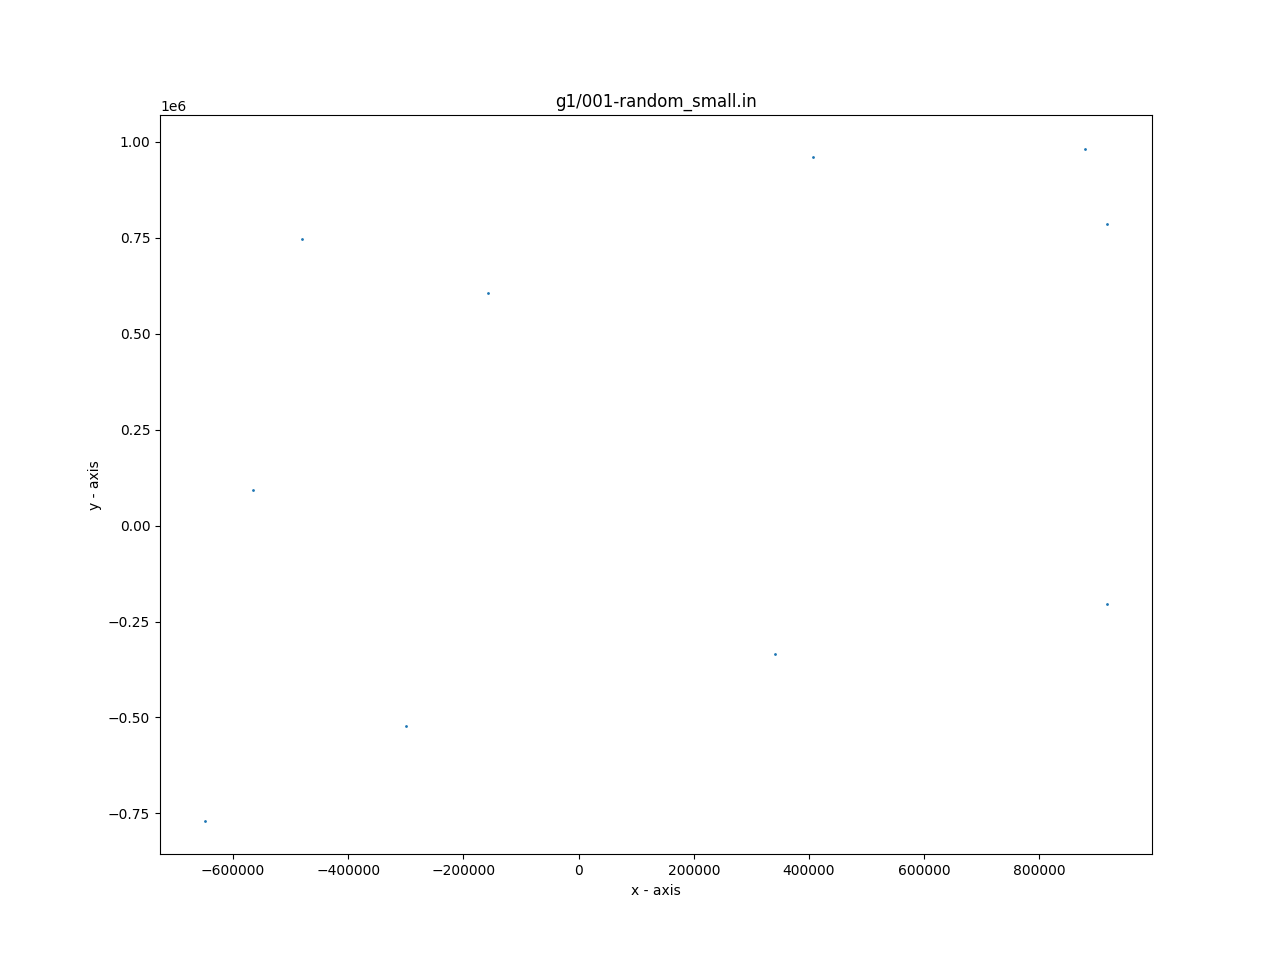
\includegraphics[scale=0.4]{code/visualizer/testdata/01.png}
	\caption{Test case 1 plotted on a coordinate plane.}
	\label{fig:01}
\end{figure}
\begin{figure}[H]
	\centering
	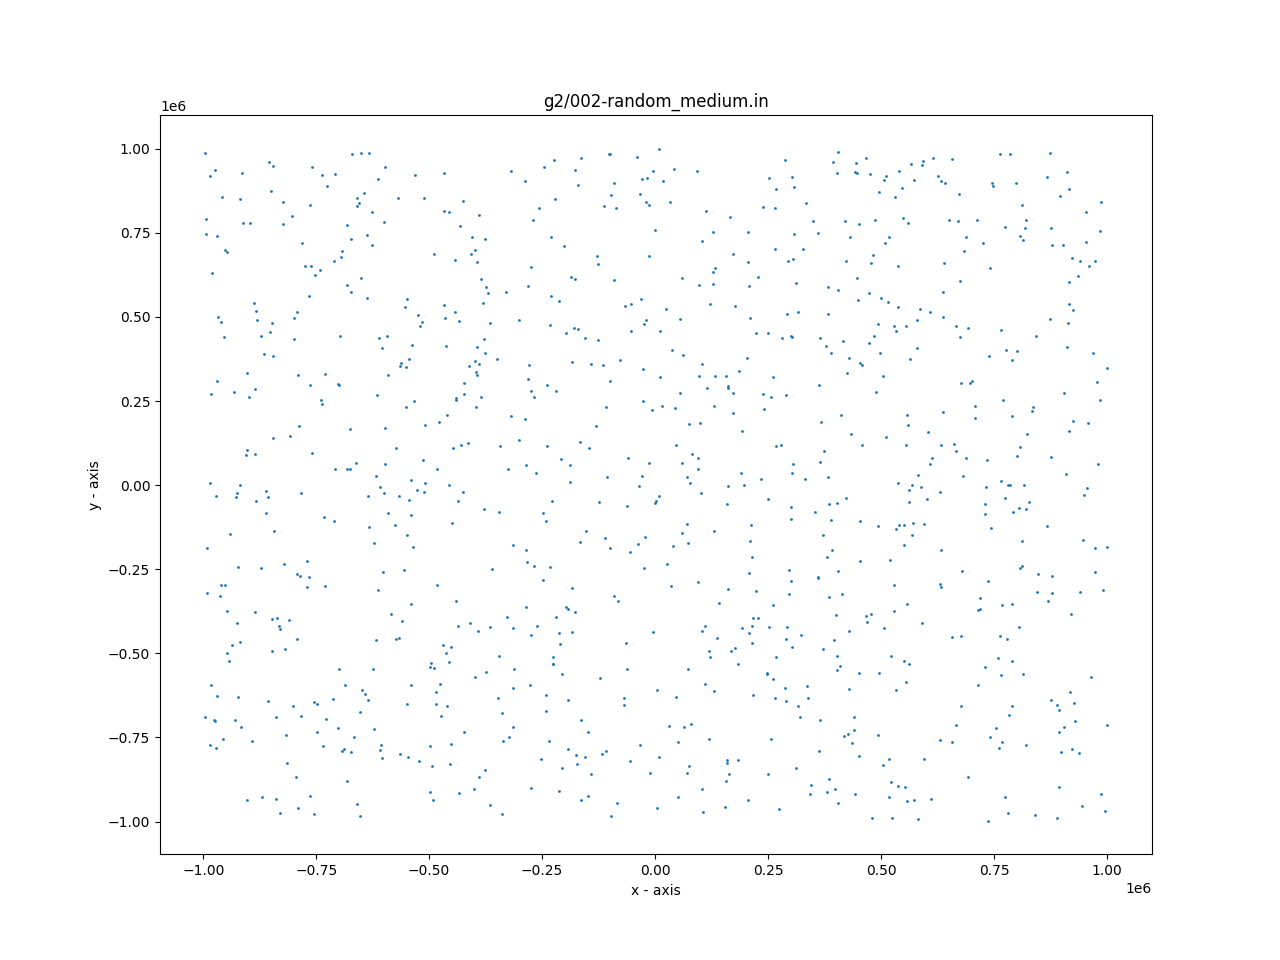
\includegraphics[scale=0.4]{code/visualizer/testdata/02.png}
	\caption{Test case 2 plotted on a coordinate plane.}
	\label{fig:02}
\end{figure}
\begin{figure}[H]
	\centering
	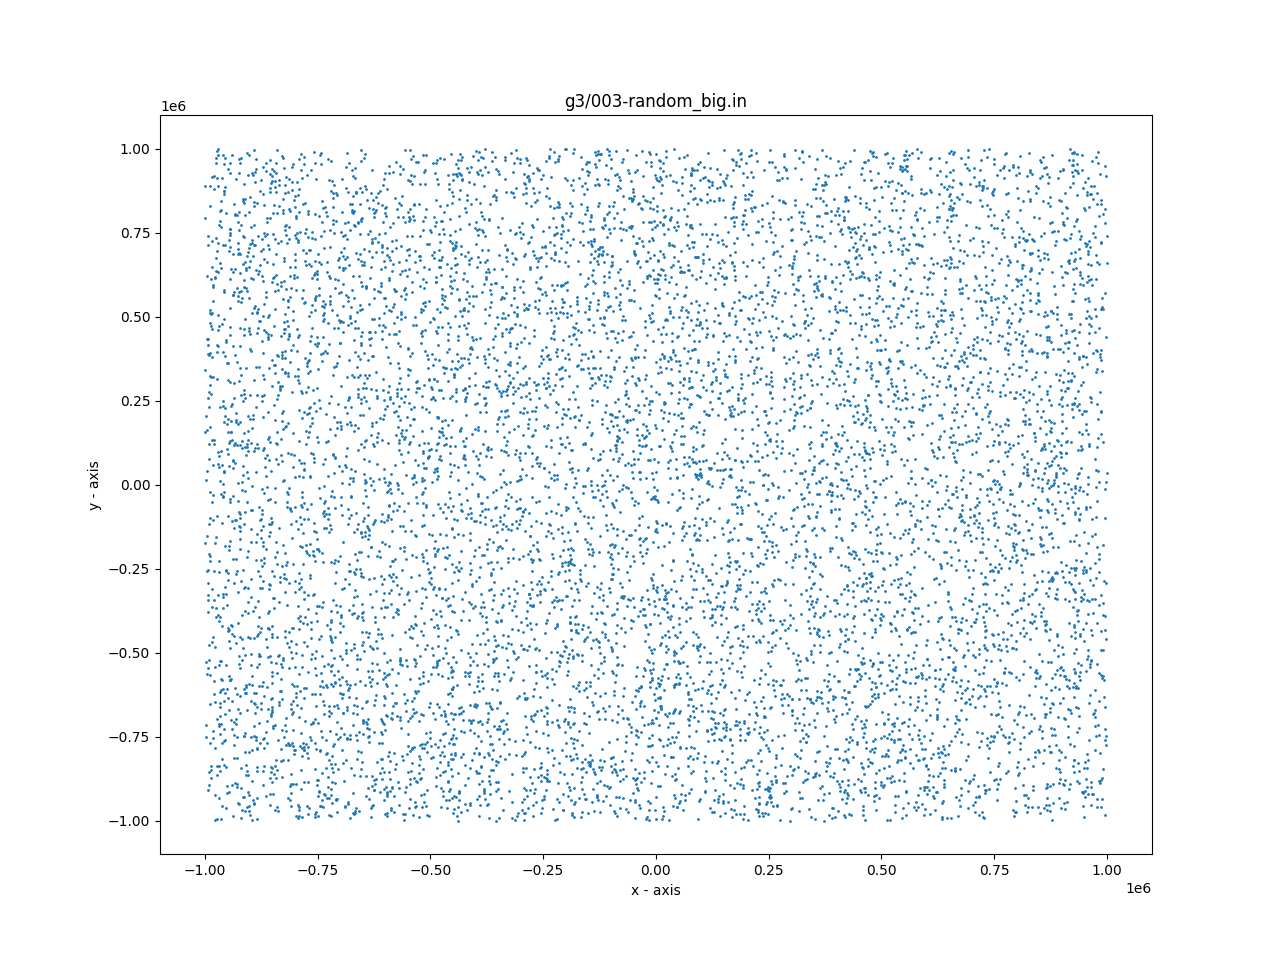
\includegraphics[scale=0.4]{code/visualizer/testdata/03.png}
	\caption{Test case 3 plotted on a coordinate plane.}
	\label{fig:03}
\end{figure}
\begin{figure}[H]
	\centering
	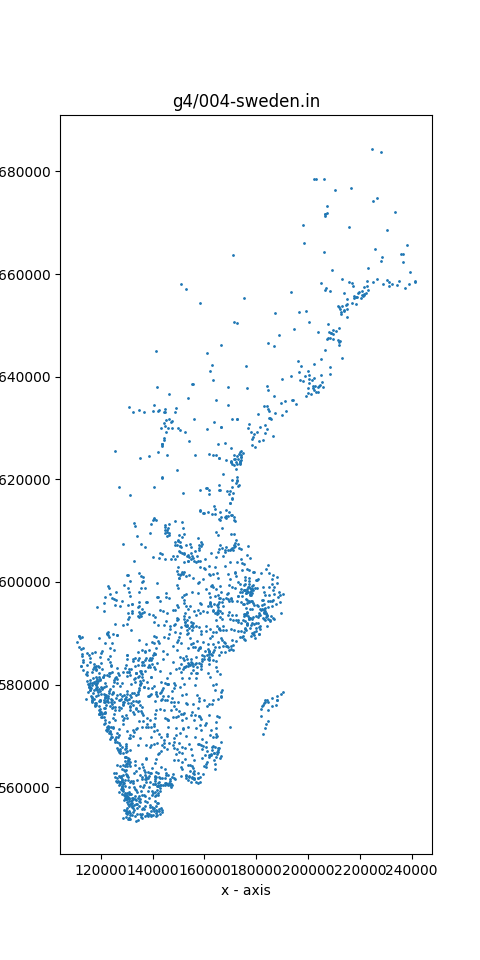
\includegraphics[scale=0.5]{code/visualizer/testdata/04.png}
	\caption{Test case 4 plotted on a coordinate plane.}
	\label{fig:04}
\end{figure}
\begin{figure}[H]
	\centering
	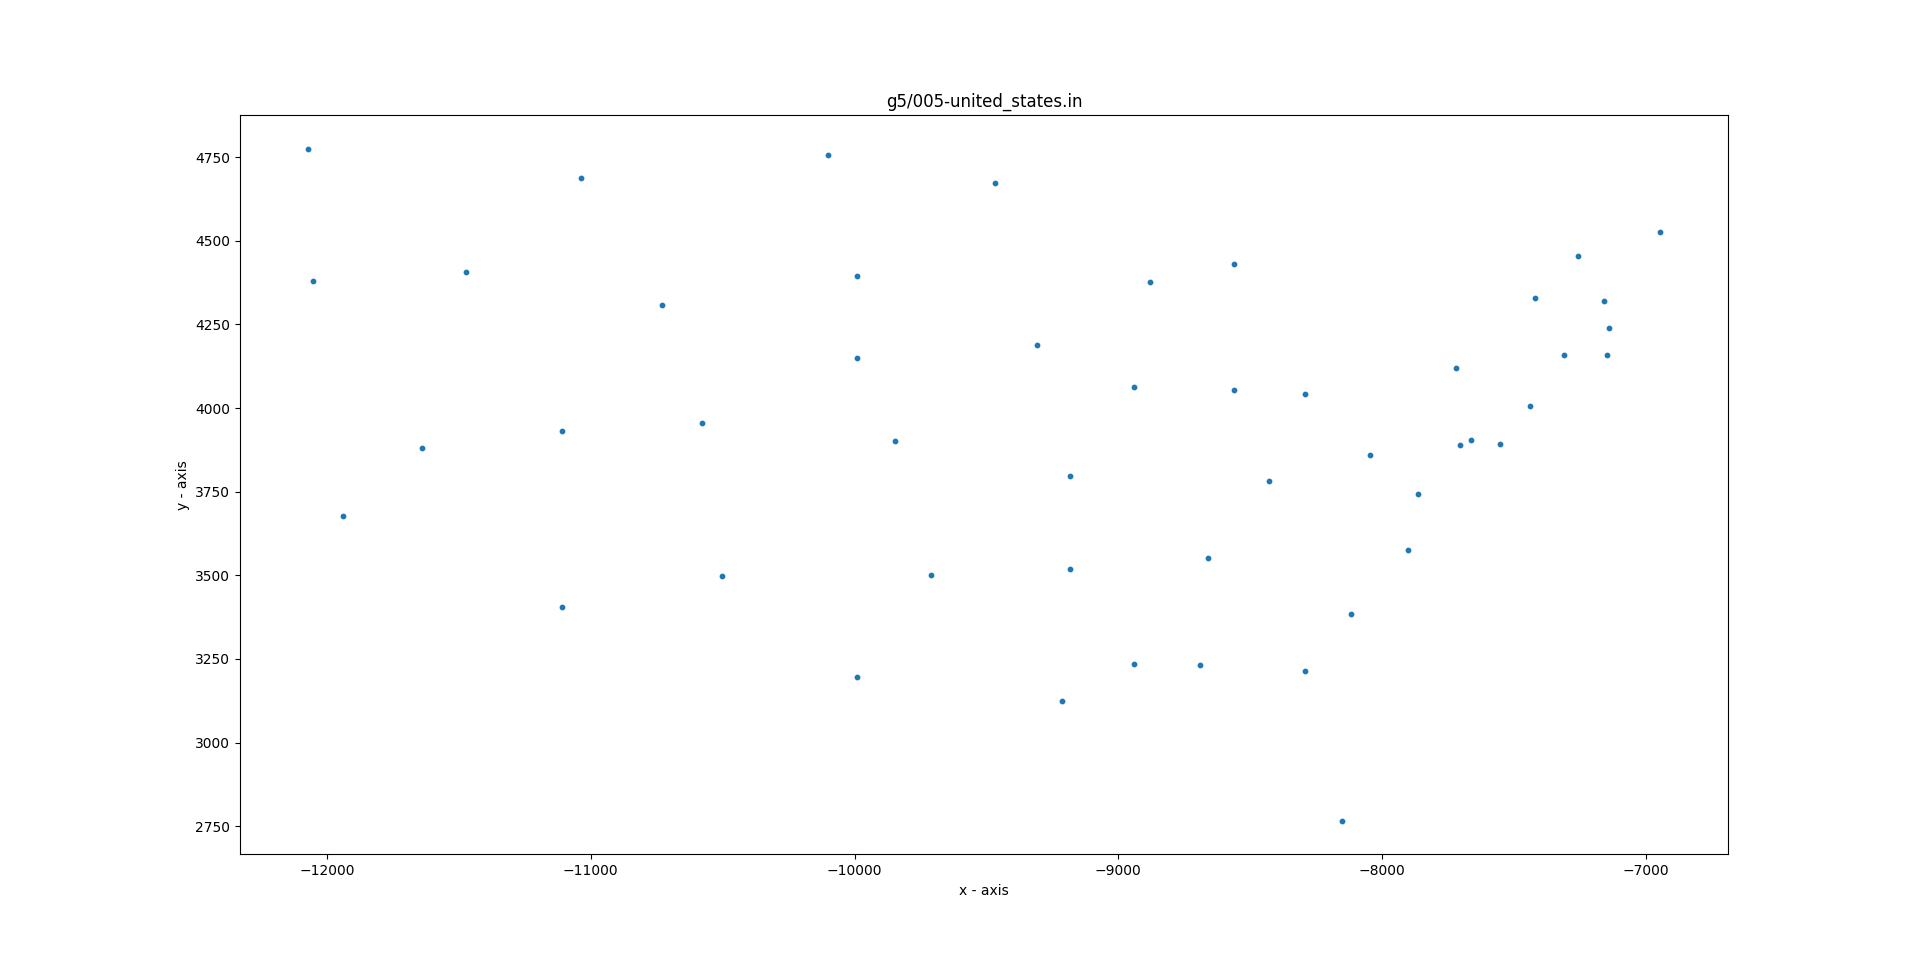
\includegraphics[scale=0.4]{code/visualizer/testdata/05.png}
	\caption{Test case 5 plotted on a coordinate plane.}
	\label{fig:05}
\end{figure}
\begin{figure}[H]
	\centering
	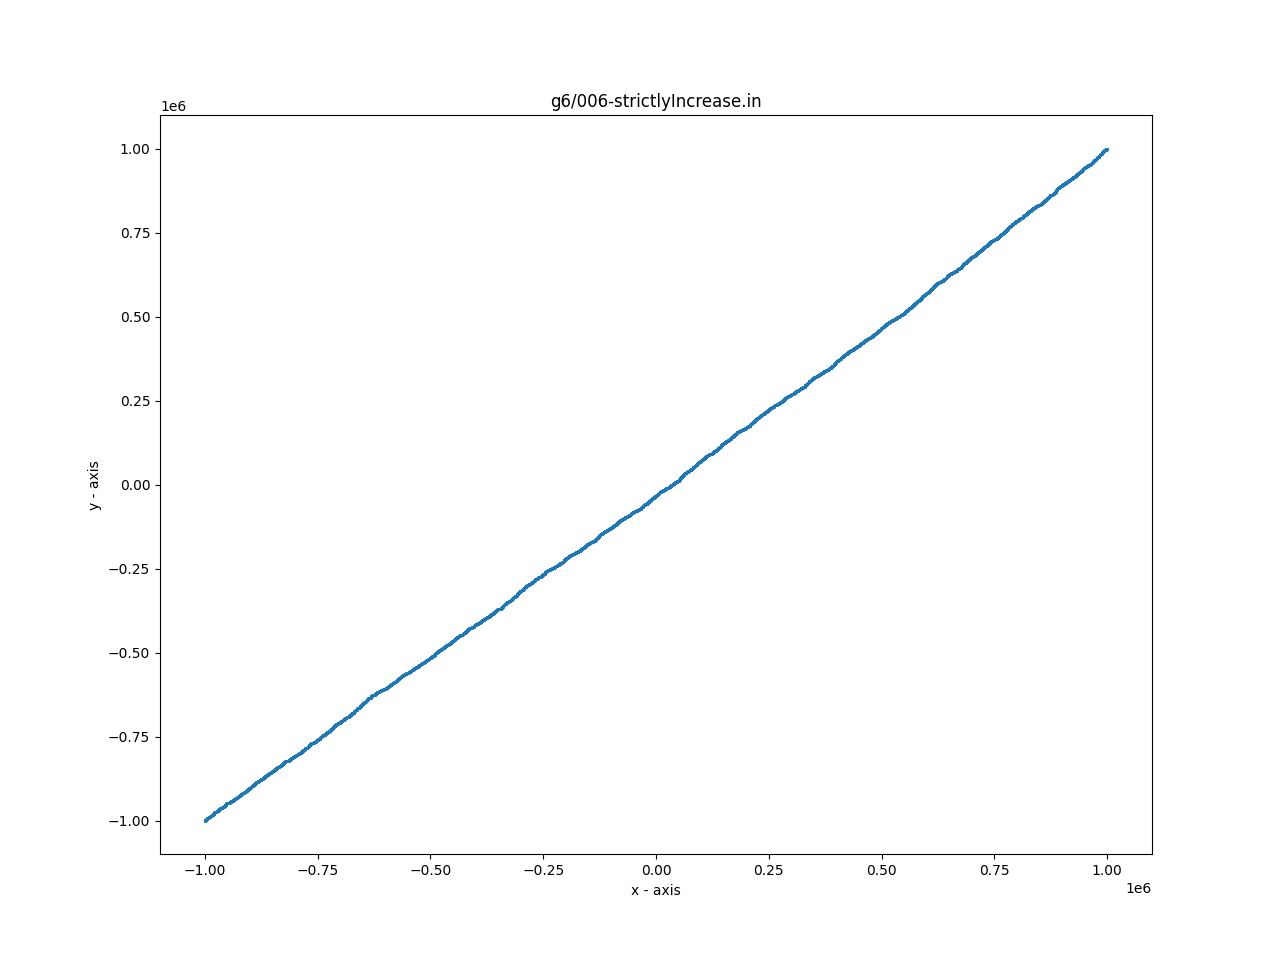
\includegraphics[scale=0.38]{code/visualizer/testdata/06.png}
	\caption{Test case 6 plotted on a coordinate plane.}
	\label{fig:06}
\end{figure}
\begin{figure}[H]
	\centering
	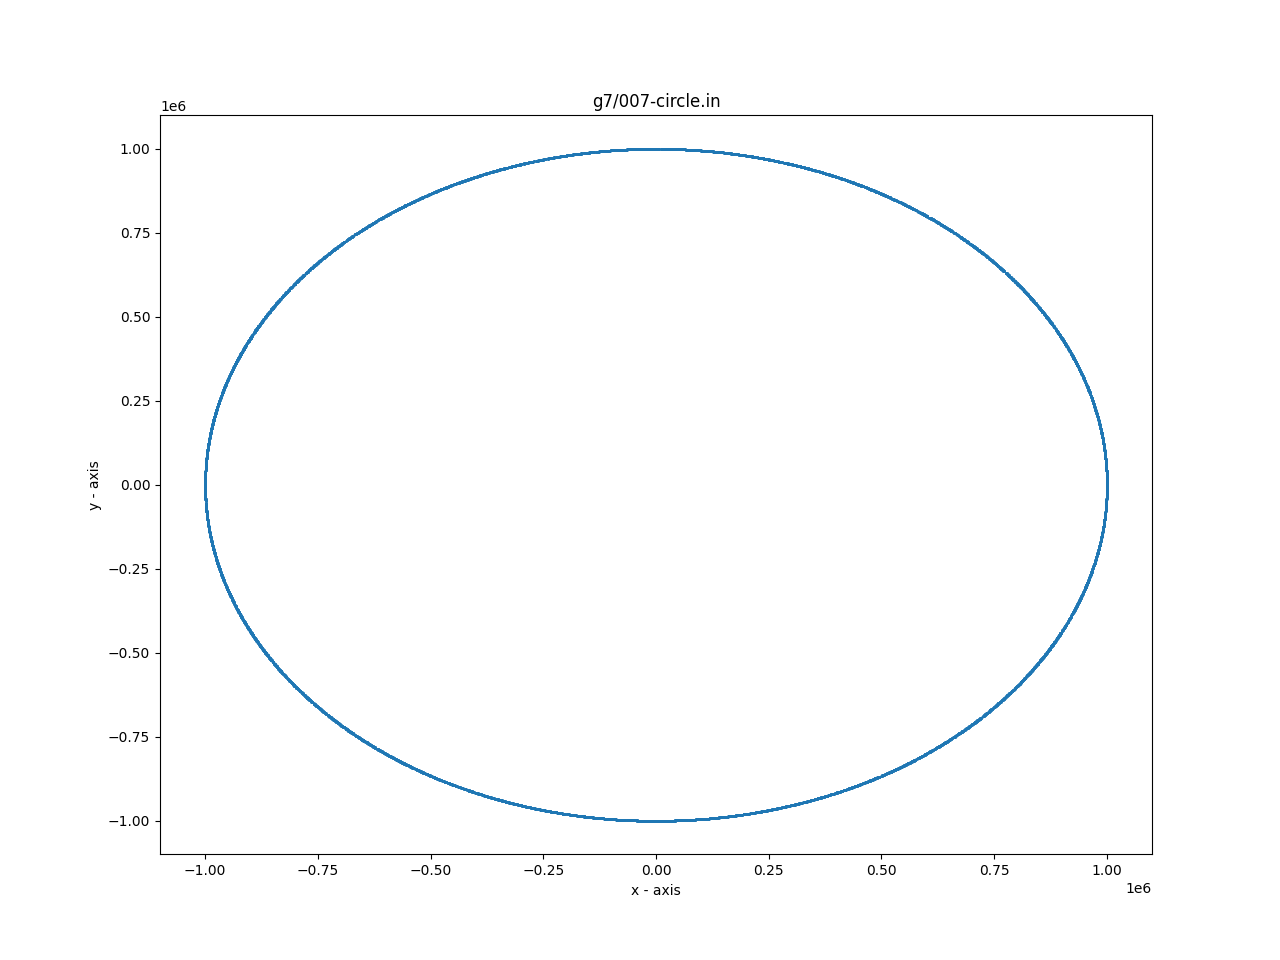
\includegraphics[scale=0.4]{code/visualizer/testdata/07.png}
	\caption{Test case 7 plotted on a coordinate plane.}
	\label{fig:07}
\end{figure}
\begin{figure}[H]
	\centering
	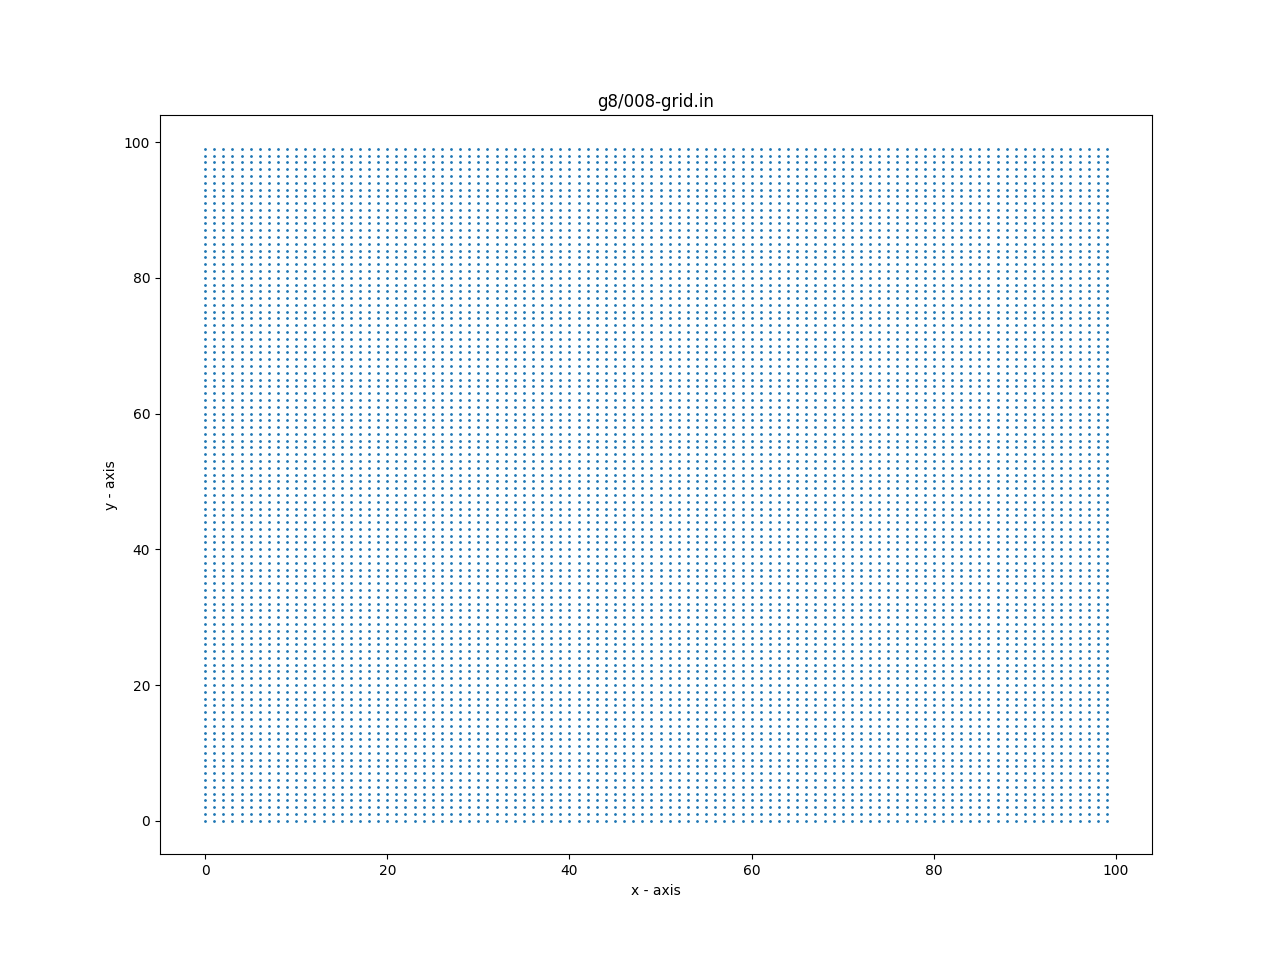
\includegraphics[scale=0.4]{code/visualizer/testdata/08.png}
	\caption{Test case 8 plotted on a coordinate plane.}
	\label{fig:08}
\end{figure}
\begin{figure}[H]
	\centering
	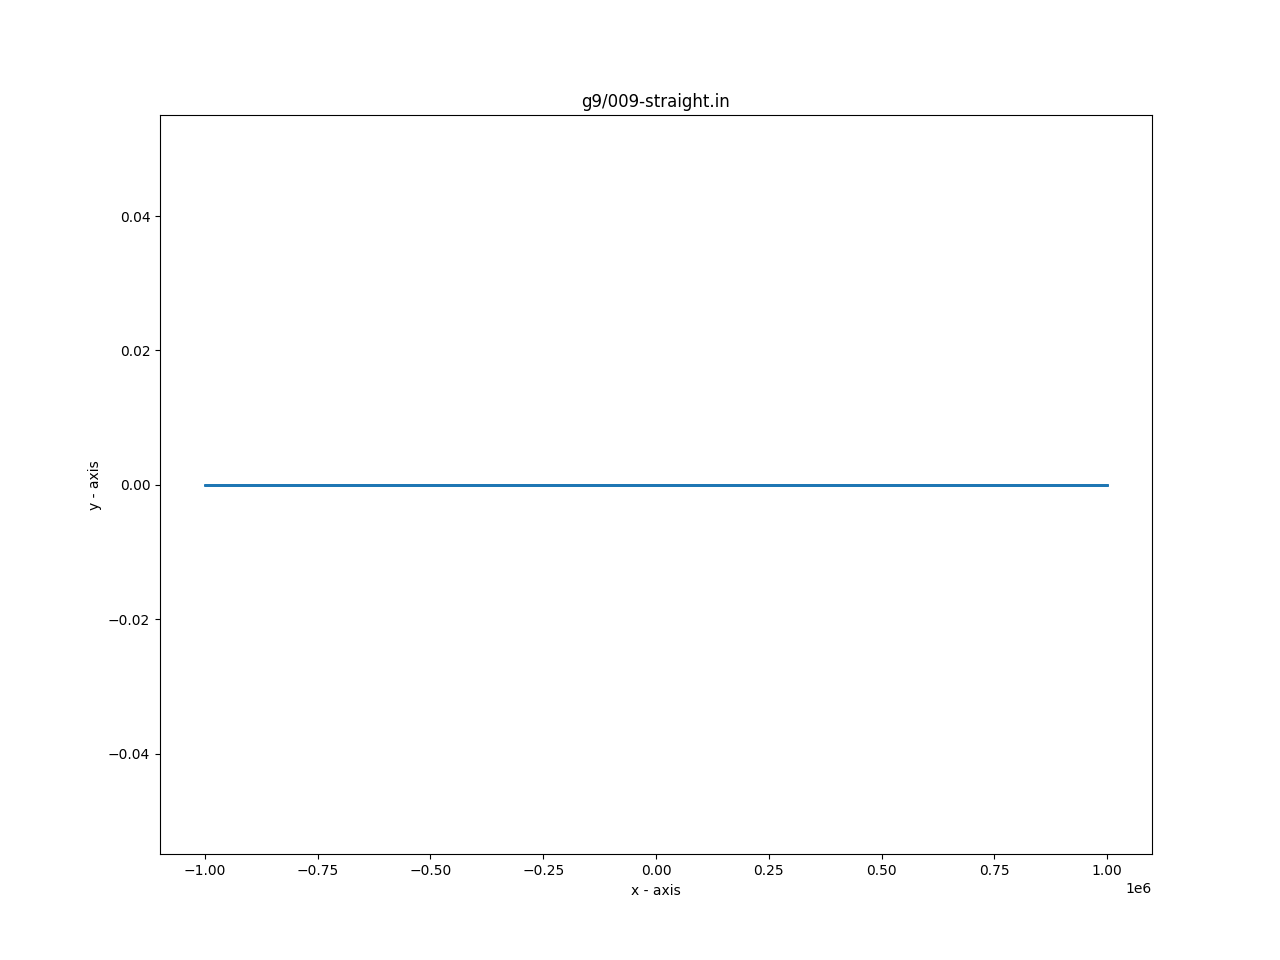
\includegraphics[scale=0.4]{code/visualizer/testdata/09.png}
	\caption{Test case 9 plotted on a coordinate plane.}
	\label{fig:09}
\end{figure}
\begin{figure}[H]
	\centering
	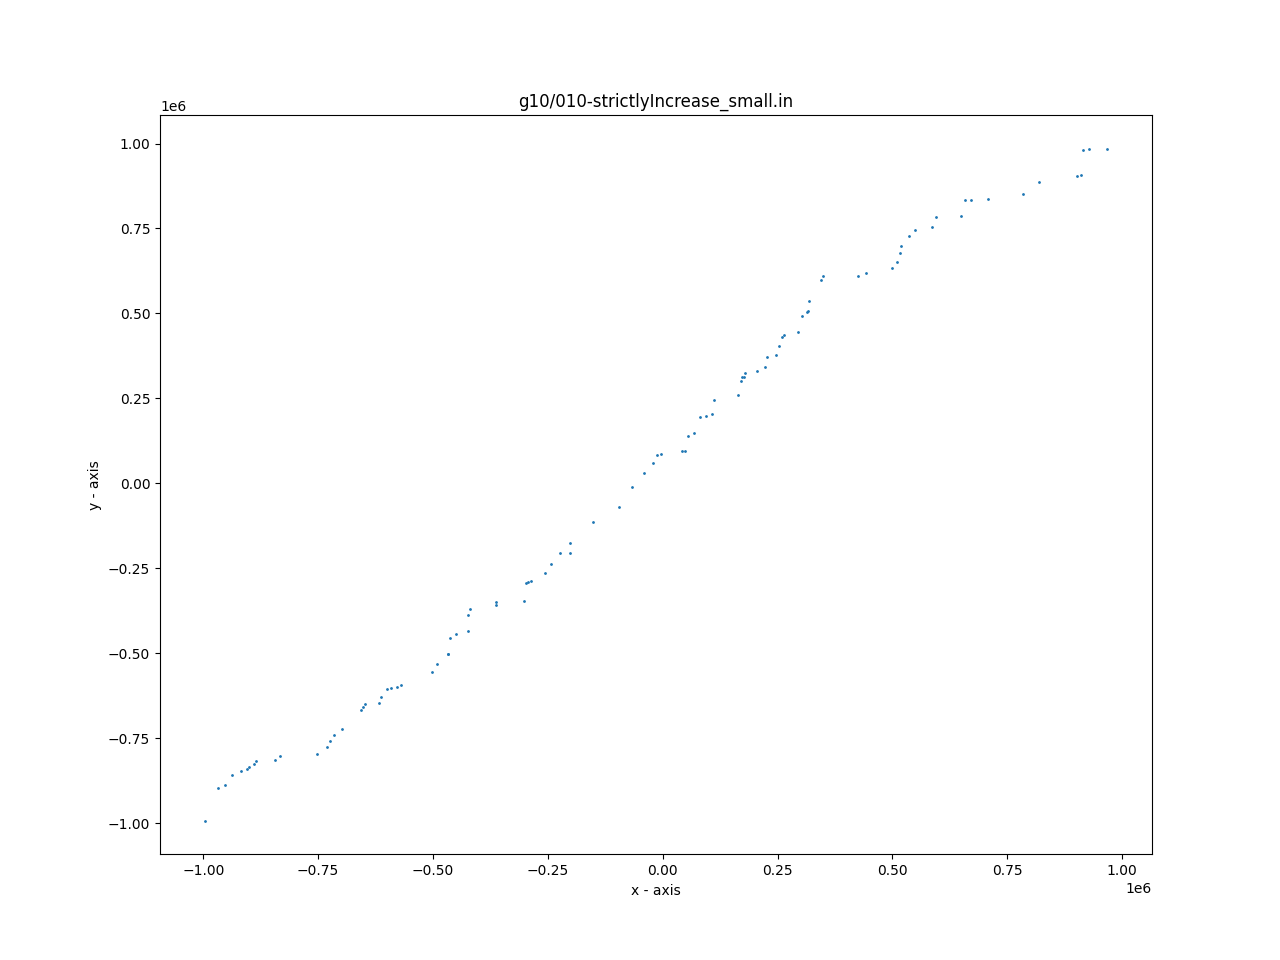
\includegraphics[scale=0.4]{code/visualizer/testdata/10.png}
	\caption{Test case 10 plotted on a coordinate plane.}
	\label{fig:10}
\end{figure}

\newpage
\section{Raw Results}
\label{appendix:RawResults}

\begin{table}[H]
    \caption{Shortest path found from each run when run on Map 1. Random generation algorithm, modified Dijkstra's algorithm, genetic random swapping algorithm, and genetic 2-opt swapping algorithm were used. The values are distance values, which are the total length of the shortest path found after the algorithm was run for 2 seconds. Values are given in units of length.}\label{Table Map 1}
    \centering
    \begin{tabular}{|p{0.2\linewidth}|p{0.2\linewidth}|p{0.2\linewidth}|p{0.2\linewidth}|}
    \hline
        \textbf{Map 1} & ~ & ~ & ~ \\ \hline
        \textbf{Random Gen} & \textbf{Modified Dijkstra's} & \textbf{Random Swapping} & \textbf{2-opt Swapping} \\ \hline
        5891573.876 & 5891573.876 & 5891573.876 & 5891573.876 \\ \hline
        5891573.876 & 5891573.876 & 5891573.876 & 5891573.876 \\ \hline
        5891573.876 & 5891573.876 & 5891573.876 & 5891573.876 \\ \hline
        5891573.876 & 5891573.876 & 5891573.876 & 5891573.876 \\ \hline
        5891573.876 & 5891573.876 & 5891573.876 & 5891573.876 \\ \hline
        6131798.700 & 5891573.876 & 5891573.876 & 5891573.876 \\ \hline
    \end{tabular}
\end{table}

\begin{table}[H]
    \caption{Shortest path found from each run when run on Map 2. Random generation algorithm, modified Dijkstra's algorithm, genetic random swapping algorithm, and genetic 2-opt swapping algorithm were used. The values are distance values, which are the total length of the shortest path found after the algorithm was run for 2 seconds. Values are given in units of length.}
    \centering
    \begin{tabular}{|p{0.2\linewidth}|p{0.2\linewidth}|p{0.2\linewidth}|p{0.2\linewidth}|}
    \hline
        \textbf{Map 2} & ~ & ~ & ~ \\ \hline
        \textbf{Random Gen} & \textbf{Modified Dijkstra's} & \textbf{Random Swapping} & \textbf{2-opt Swapping} \\ \hline
        992924716.9 & 375916823.6 & 225977937.9 & 72516889.45 \\ \hline
        987691105.0 & 372737685.5 & 229849151.6 & 69427895.87 \\ \hline
        995151465.5 & 369072515.4 & 221449499.6 & 68808723.25 \\ \hline
        989088278.2 & 371810727.2 & 232695937.3 & 69720673.41 \\ \hline
        989255767.2 & 373373480.0 & 233207053.9 & 70331677.81 \\ \hline
        991826128.7 & 373281345.9 & 207510610.3 & 69670533.67 \\ \hline
    \end{tabular}
\end{table}

\begin{table}[H]
    \caption{Shortest path found from each run when run on Map 3. Random generation algorithm, modified Dijkstra's algorithm, genetic random swapping algorithm, and genetic 2-opt swapping algorithm were used. The values are distance values, which are the total length of the shortest path found after the algorithm was run for 2 seconds. Values are given in units of length.}
    \centering
    \begin{tabular}{|p{0.2\linewidth}|p{0.2\linewidth}|p{0.2\linewidth}|p{0.2\linewidth}|}
    \hline
        \textbf{Map 3} & ~ & ~ & ~ \\ \hline
        \textbf{Random Gen} & \textbf{Modified Dijkstra's} & \textbf{Random Swapping} & \textbf{2-opt Swapping} \\ \hline
        10323119546 & 3240428284 & 3793530293 & 3152792905 \\ \hline
        10279776945 & 3233877905 & 3776841645 & 2937278015 \\ \hline
        10298645329 & 3234864733 & 3822141990 & 3095200214 \\ \hline
        10298914814 & 3234688577 & 3842225040 & 3020962352 \\ \hline
        10285436723 & 3228157454 & 3828077792 & 2984305232 \\ \hline
        10300080362 & 3232665916 & 3807533962 & 3049464688 \\ \hline
    \end{tabular}
\end{table}

\begin{table}[H]
    \caption{Shortest path found from each run when run on Map 4. Random generation algorithm, modified Dijkstra's algorithm, genetic random swapping algorithm, and genetic 2-opt swapping algorithm were used. The values are distance values, which are the total length of the shortest path found after the algorithm was run for 2 seconds. Values are given in units of length.} \label{Table Map 4}
    \centering
    \begin{tabular}{|p{0.2\linewidth}|p{0.2\linewidth}|p{0.2\linewidth}|p{0.2\linewidth}|}
    \hline
        \textbf{Map 4} & ~ & ~ & ~ \\ \hline
        \textbf{Random Gen} & \textbf{Modified Dijkstra's} & \textbf{Random Swapping} & \textbf{2-opt Swapping} \\ \hline
        79693630.34 & 27564839.82 & 20262321.82 & 6084857.948 \\ \hline
        79693630.34 & 27473123.85 & 19561130.69 & 6204447.677 \\ \hline
        79693630.34 & 27566245.04 & 19480924.30 & 5934914.712 \\ \hline
        79693630.34 & 27734229.92 & 19246108.98 & 5871981.884 \\ \hline
        79693630.34 & 27636185.38 & 20044024.37 & 5924928.645 \\ \hline
        79693630.34 & 27755956.26 & 19643845.39 & 6129804.537 \\ \hline
    \end{tabular}
\end{table}

\begin{table}[H]
    \caption{Shortest path found from each run when run on Map 5. Random generation algorithm, modified Dijkstra's algorithm, genetic random swapping algorithm, and genetic 2-opt swapping algorithm were used. The values are distance values, which are the total length of the shortest path found after the algorithm was run for 2 seconds. Values are given in units of length.}
    \centering
    \begin{tabular}{|p{0.2\linewidth}|p{0.2\linewidth}|p{0.2\linewidth}|p{0.2\linewidth}|}
    \hline
        \textbf{Map 5} & ~ & ~ & ~ \\ \hline
        \textbf{Random Gen} & \textbf{Modified Dijkstra's} & \textbf{Random Swapping} & \textbf{2-opt Swapping} \\ \hline
        63470.66185 & 32761.02342 & 23363.90715 & 18288.09154 \\ \hline
        63890.85113 & 31608.69660 & 23739.19883 & 18205.12660 \\ \hline
        64490.25890 & 31536.60587 & 21482.12635 & 18234.21287 \\ \hline
        62379.14452 & 31131.14313 & 22779.03298 & 18311.86805 \\ \hline
        66385.01545 & 31806.52710 & 23763.20389 & 18311.86805 \\ \hline
        60399.75765 & 31211.23317 & 20760.25464 & 18300.61299 \\ \hline
     \end{tabular}
\end{table}

\begin{table}[H]
    \caption{Shortest path found from each run when run on Map 6. Random generation algorithm, modified Dijkstra's algorithm, genetic random swapping algorithm, and genetic 2-opt swapping algorithm were used. The values are distance values, which are the total length of the shortest path found after the algorithm was run for 2 seconds. Values are given in units of length.}
    \centering
    \begin{tabular}{|p{0.2\linewidth}|p{0.2\linewidth}|p{0.2\linewidth}|p{0.2\linewidth}|}
    \hline
        \textbf{Map 6} & ~ & ~ & ~ \\ \hline
        \textbf{Random Gen} & \textbf{Modified Dijkstra's} & \textbf{Random Swapping} & \textbf{2-opt Swapping} \\ \hline
        9291380109 & 1349024996 & 2373586959 & 1814447149 \\ \hline
        9310437819 & 1348572833 & 2280159165 & 1455553611 \\ \hline
        9297883462 & 1357296776 & 2344747004 & 1601361008 \\ \hline
        9302381835 & 1353080817 & 2306799937 & 1599620455 \\ \hline
        9286799450 & 1350374546 & 2325432171 & 1593378825 \\ \hline
        9329019143 & 1348033186 & 2361945269 & 1646813150 \\ \hline
    \end{tabular}
\end{table}

\begin{table}[H]
    \caption{Shortest path found from each run when run on Map 7. Random generation algorithm, modified Dijkstra's algorithm, genetic random swapping algorithm, and genetic 2-opt swapping algorithm were used. The values are distance values, which are the total length of the shortest path found after the algorithm was run for 2 seconds. Values are given in units of length.}
    \centering
    \begin{tabular}{|p{0.2\linewidth}|p{0.2\linewidth}|p{0.2\linewidth}|p{0.2\linewidth}|}
    \hline
        \textbf{Map 7} & ~ & ~ & ~ \\ \hline
        \textbf{Random Gen} & \textbf{Modified Dijkstra's} & \textbf{Random Swapping} & \textbf{2-opt Swapping} \\ \hline
        12567650338 & 2248980912 & 3908157889 & 2537013830 \\ \hline
        12573745599 & 2217757665 & 3952339027 & 2431780351 \\ \hline
        12600808851 & 2244295348 & 3929417131 & 2620719310 \\ \hline
        12577611347 & 2237577332 & 3851583858 & 2445124971 \\ \hline
        12549889305 & 2238673128 & 3951409612 & 2557729463 \\ \hline
        12551595182 & 2245565916 & 3884563307 & 2602087504 \\ \hline
    \end{tabular}
\end{table}

\begin{table}[H]
    \caption{Shortest path found from each run when run on Map 8. Random generation algorithm, modified Dijkstra's algorithm, genetic random swapping algorithm, and genetic 2-opt swapping algorithm were used. The values are distance values, which are the total length of the shortest path found after the algorithm was run for 2 seconds. Values are given in units of length.}
    \centering
    \begin{tabular}{|p{0.2\linewidth}|p{0.2\linewidth}|p{0.2\linewidth}|p{0.2\linewidth}|}
    \hline
        \textbf{Map 8} & ~ & ~ & ~ \\ \hline
        \textbf{Random Gen} & \textbf{Modified Dijkstra's} & \textbf{Random Swapping} & \textbf{2-opt Swapping} \\ \hline
        516272.1618 & 162933.9379 & 189487.4362 & 146595.3781 \\ \hline
        515198.6725 & 162480.3180 & 185568.5141 & 148485.5344 \\ \hline
        515030.9863 & 162150.3042 & 186938.2779 & 148197.8332 \\ \hline
        516285.3527 & 162161.4700 & 186978.8585 & 148080.8074 \\ \hline
        513969.2742 & 161665.9353 & 184770.9426 & 142505.3975 \\ \hline
        514867.3062 & 162288.9124 & 186445.5991 & 148529.9744 \\ \hline
    \end{tabular}
\end{table}

\begin{table}[H]
    \caption{Shortest path found from each run when run on Map 9. Random generation algorithm, modified Dijkstra's algorithm, genetic random swapping algorithm, and genetic 2-opt swapping algorithm were used. The values are distance values, which are the total length of the shortest path found after the algorithm was run for 2 seconds. Values are given in units of length.}
    \centering
    \begin{tabular}{|p{0.2\linewidth}|p{0.2\linewidth}|p{0.2\linewidth}|p{0.2\linewidth}|}
    \hline
        \textbf{Map 9} & ~ & ~ & ~ \\ \hline
        \textbf{Random Gen} & \textbf{Modified Dijkstra's} & \textbf{Random Swapping} & \textbf{2-opt Swapping} \\ \hline
        6553370088 & 949184378 & 1656974798 & 896028426 \\ \hline
        6565113386 & 946308942 & 1643517954 & 903780140 \\ \hline
        6506833168 & 961167540 & 1620169650 & 808419124 \\ \hline
        6545958006 & 945003364 & 1668749822 & 787330814 \\ \hline
        6535809660 & 956124694 & 1613793366 & 806036378 \\ \hline
        6562710126 & 951048114 & 1582440390 & 779322396 \\ \hline
    \end{tabular}
\end{table}

\begin{table}[H]
    \caption{Shortest path found from each run when run on Map 10. Random generation algorithm, modified Dijkstra's algorithm, genetic random swapping algorithm, and genetic 2-opt swapping algorithm were used. The values are distance values, which are the total length of the shortest path found after the algorithm was run for 2 seconds. Values are given in units of length.}
    \centering
    \begin{tabular}{|p{0.2\linewidth}|p{0.2\linewidth}|p{0.2\linewidth}|p{0.2\linewidth}|}
    \hline
        \textbf{Map 10} & ~ & ~ & ~ \\ \hline
        \textbf{Random Gen} & \textbf{Modified Dijkstra's} & \textbf{Random Swapping} & \textbf{2-opt Swapping} \\ \hline
        67609575.19 & 20823427.49 & 11069509.51 & 5815136.523 \\ \hline
        69664811.60 & 20805907.35 & 11533087.55 & 5810589.705 \\ \hline
        67715528.88 & 20874288.90 & 10755444.78 & 5804089.746 \\ \hline
        68228851.14 & 21454217.01 & 12453953.00 & 5792401.336 \\ \hline
        68862987.39 & 19999070.68 & 12382933.57 & 5812265.150 \\ \hline
        70379810.37 & 21192230.70 & 10883480.63 & 5800222.750 \\ \hline
    \end{tabular}
\end{table}


\end{appendices}

\end{document}
